
\documentclass[reprint,amsmath,amssymb,
 aps]{revtex4-2}

\usepackage{graphicx}% Include figure files
\usepackage{dcolumn}% Align table columns on decimal point
\usepackage{bm}% bold math
\usepackage{subcaption}
\usepackage{color}
\usepackage{enumerate}
\usepackage{mathtools}
\usepackage[hidelinks,pdfusetitle,pdfdisplaydoctitle]{hyperref}
\usepackage[capitalise]{cleveref}
% To make pretty tables
\usepackage{booktabs}
\usepackage{multirow}

% useful commands
\newcommand{\bn}{\bold{n}}
\newcommand{\bx}{\boldsymbol{x}}
\newcommand{\bh}[1]{\bold{\hat{#1}}}
\newcommand{\bhx}{{\bold{\hat{x}}}}
\newcommand{\bhy}{\bold{\hat{y}}}
\newcommand{\hx}{{\hat{x}}}
\newcommand{\hy}{{\hat{y}}}
\newcommand{\hvarphi}{{\hat{\varphi}}}
\newcommand{\hPhi}{{\hat{\Phi}}}
\newcommand{\by}{\boldsymbol{y}}
\newcommand{\br}{\boldsymbol{r}}
\newcommand{\btheta}{\bold{\theta}}
\newcommand{\htau}{{\hat{\tau}}}
\newcommand{\hpsi}{{\hat{\psi}}}
\newcommand{\M}{\mathcal{T}}
\newcommand{\chia}{\chi^{\text{affine}}}
\newcommand{\pt}{\bold{P}}
\newcommand{\uapprox}{u^{\text{approx}}}
\newcommand{\uref}{u^{\text{ref}}}

\newcommand{\bol}{\boldsymbol}
\newcommand{\nee}{\bold{e}}
\newcommand{\nej}{\bold{j}}
\newcommand{\nem}{\bold{m}}
\newcommand{\nephi}{\boldsymbol{\phi}}
\newcommand{\nepsi}{\boldsymbol{\psi}}
\newcommand{\new}{\boldsymbol w}
\newcommand{\ney}{\boldsymbol{y}}
\newcommand{\nex}{\boldsymbol{x}}
\newcommand{\bnex}{\bold{x}}
\newcommand{\nez}{\boldsymbol{z}}
\newcommand{\nev}{\boldsymbol{v}}
\newcommand{\neu}{\boldsymbol{u}}
\newcommand{\nerho}{\boldsymbol{\varrho}}
\newcommand{\ner}{\bol{r}}
\newcommand{\TE}{\mathrm{TE}}
\newcommand{\TM}{\mathrm{TM}}
\newcommand{\de}{\,\mathrm{d}}
\newcommand{\e}{\operatorname{e}}
\newcommand{\im}{\operatorname{i}}
\newcommand{\inc}{\mathrm{inc}}
\newcommand{\rad}{\mathrm{rad}}
\newcommand{\gui}{\mathrm{gui}}
\newcommand{\ontext}{\quad\mbox{on}\quad}
\newcommand{\intext}{\quad\mbox{in}\quad}
\newcommand{\andtext}{\quad\mbox{and}\quad}
\newcommand{\dtn}{\mathcal{B}}
\newcommand{\dtnn}{\mathrm{T}}
\newcommand{\sovo}{\operatorname{H}}
\newcommand{\keps}{k_{\varepsilon}}
\newcommand{\p}{\partial}
\newcommand{\mpt}{\mathbf A}
\newcommand{\crt}{\mathbf J}
\newcommand{\dygfn}{\bar{\bold G}}
\newcommand{\untx}{\hat x}
\newcommand{\unty}{\hat y}
\newcommand{\untz}{\hat z}
\newcommand{\teps}{\boldsymbol{\overline\epsilon}}
\newcommand{\tmu}{\boldsymbol{\overline\mu}}
\newcommand{\ftr}{\widehat{F}}
\newcommand{\dlpfs}{\bold{K}^{\mathrm{fs}}}
\newcommand{\dlphs}{\bold{K}^{\mathrm{hs}}}
\newcommand{\slpfs}{\bold{S}^{\mathrm{fs}}}
\newcommand{\slphs}{\bold{S}^{\mathrm{hs}}}
\newcommand{\real}{\mathrm{Re}\,}
\newcommand{\uinc}{u_{\mathrm{inc}}}
\newcommand{\imag}{\mathrm{Im}\,}
\newcommand{\inte}{\mathrm{int}}
\newcommand{\exte}{\mathrm{ext}}
\newcommand{\lf}{\left}
\newcommand{\rg}{\right}
\newcommand{\tdir}{\widehat{\boldsymbol \theta}}
\newcommand{\rdir}{\widehat{\boldsymbol r}}
\newcommand{\xdir}{\widehat{\bold i}}
\newcommand{\ydir}{\widehat{\bold j}}
\newcommand{\zdir}{\widehat{\bold k}}
\newcommand{\R}{\mathbb{R}}
\newcommand{\C}{\mathbb{C}}
\newcommand{\N}{\mathbb{N}}
\newcommand{\Z}{\mathbb{Z}}
\newcommand{\elc}{\mathbf E}
\newcommand{\mgn}{\mathbf H}
\newcommand{\mgf}{\bold H}
\newcommand{\elf}{\bold E}
\newcommand{\can}{\bold e}
\newcommand{\normal}{n}
\newcommand{\nor}{\bold n}
\newcommand{\curl}{\operatorname{curl}}
\newcommand{\grd}{\operatorname{grad}}
\newcommand{\dv}{\operatorname{div}}
\newcommand{\vecphi}{\boldsymbol{\upphi}}

\newcommand{\Dcal}{\mathcal{D}}
\newcommand{\Bcal}{\mathcal{B}}
\newcommand{\Gcal}{\mathcal{G}}
\newcommand{\Hcal}{\mathcal{H}}
\newcommand{\Ical}{\mathcal{I}}
\newcommand{\Lcal}{\mathcal{L}}
\newcommand{\Mcal}{\mathcal{M}}
\newcommand{\Ocal}{\mathcal{O}}
\newcommand{\Pcal}{\mathcal{P}}
\newcommand{\Qcal}{\mathcal{Q}}
\newcommand{\Scal}{\mathcal{S}}
\newcommand{\Wcal}{\mathcal{W}}
\newcommand{\Tcal}{\mathcal{T}}
\newcommand{\Vcal}{\mathcal{V}}
\newcommand{\Kcal}{\mathcal{K}}
\newcommand{\tG}{\mathbb{G}}
\newcommand{\tId}{\mathbb{I}}

\newcommand{\bigo}[1]{\Ocal\left(#1\right)}
\newcommand{\abs}[1]{\left|#1\right|}
\newcommand{\norm}[1]{\left\|#1\right\|}
\newcommand\inner[1]{\left\langle#1\right\rangle}
\renewcommand{\quote}[1]{``#1''}

\begin{document}

%\preprint{APS/123-QED}

\title{Implementation of the Boundary Integral Equation Neumann-to-Dirichlet map (BIE-NtD) method for the analysis of 1D-periodic diffraction gratings}

\author{Rodrigo Arrieta}
\altaffiliation{Mathematics
 Department, Massachusetts Institute of Technology, Cambridge, MA 02139, United
States}
\email{rarrieta@mit.edu}

\date{\today}% It is always \today, today,
             %  but any date may be explicitly specified

\begin{abstract}
This report presents an implementation of the BIE-NtD method, as proposed by Wu and Lu (2009), for computing transmission and reflection coefficients of 1D-periodic diffraction gratings and photonic crystal (PhC) slabs. The approach totally bypasses the use of the problematic quasiperiodic Green's function, employing the free-space Green's function instead. We establish an analogy between this method and the Transfer Matrix Method (TMM) for planar isotropic layered media, identifying the BIE-NtD method as a direct generalization of the TMM for isotropic layered media with periodic interfaces. Furthermore, various examples demonstrating the application of the BIE-NtD method are showcased. We finally mention some potential suggestions to improve the speed and efficiency of the method.
\end{abstract}

%\keywords{Suggested keywords}%Use showkeys class option if keyword
                              %display desired
\maketitle

%\tableofcontents

\section{Problem formulation}\label{sec:problem_form}
We consider diffraction gratings that are periodic in the $\bh{x}$ direction, with period $L > 0$, and invariant in the $\bh{z}$ direction. The grating comprises layers of isotropic and homogeneous materials, and it is contained in the region $0 \leq y \leq D$, as depicted in \cref{fig:diff_grat}. The top ($y > D$) and bottom ($y < 0$) regions correspond also to infinite, homogeneous, and isotropic materials with permittivities $\epsilon^{(1)}$ and $\epsilon^{(2)}$, respectively. Assume that an incoming electromagnetic plane wave, propagating in the $xy$ plane, impinges on the structure from the top domain $y > 0$, giving rise to a reflected wave in the top domain $y > 0$ and a transmitted wave in the bottom domain $y < 0$. Since the problem is $z$-invariant and every $xy$ plane acts as a mirror symmetry plane, we can reduce our attention to only light polarized as transverse electric (TE or $E_z$ polarization; the electric field only has a non-zero component in the $z$ direction) or transverse magnetic (TM or $H_z$ polarization; the magnetic field only has a non-zero component in the $z$ direction). For simplicity, for the rest of this work we will focus our attention in the $E_z$ polarized case. (The BIE-NtD method described here also works for $H_z$ polarization; it requires, however, slight modifications.) Letting $u$ be the total $z$-component of the electric field, we have that $u$ satisfies the Helmholtz equation:
\begin{eqnarray}
(\Delta + k_0^2\epsilon(x,y))u(x,y) = 0,
\end{eqnarray}
where $k_0 = \omega/c$ is the free-space wavenumber, $\omega$ is the angular frequency, $c$ is the speed of light in vacuum, and $\epsilon(x,y)$ is the permittivity at point $(x,y)$. Furthermore, both $u$ and its normal derivative $\partial u/\partial n$ are continuous across the interface between different materials. 

Let the incoming plane wave coming from the top be
\begin{align}
u^{(i)}(x,y) = e^{i(\alpha_0x - \beta_0^{(1)}y)},\qquad y > D, \label{eq:incident_wave}
\end{align}
where $\alpha_0 \in [-k_0\sqrt{\epsilon^{(1)}},k_0\sqrt{\epsilon^{(1)}}]$ is the Bloch wavenumber and $\beta_0^{(1)} = \sqrt{k_0^2\epsilon^{(1)}-\alpha_0^2}$. The structure possesses discrete translational symmetry, with period $L$, in the $x$-direction, hence Bloch's theorem asserts that the Bloch wavenumber $\alpha_0$ must be preserved up to multiples of $2\pi/L$. Let
\begin{align}
\alpha_j &= \alpha_0 + j \frac{2\pi}{L},\qquad j \in \Z,\\
\beta_j^{(1,2)} &= \sqrt{k_0^2\epsilon^{(1,2)}-\alpha_j^2},
\end{align}
where the square root of a negative number is taken with a positive imaginary part. Then, the reflected and transmitted waves admit \textit{outgoing Rayleigh-Bloch expansions} of the form 
\begin{align}
u^{(r)}(x,y) =& \sum\limits_{j=-\infty}^\infty R_je^{i\lf(\alpha_jx + \beta_j^{(1)}\left(y-D\right)\rg)},\quad y > D,\label{eq:refc}\\
u^{(t)}(x,y) =& \sum\limits_{j=-\infty}^\infty T_je^{i\lf(\alpha_jx - \beta_j^{(2)}y\rg)},\quad y < 0,\label{eq:transc}
\end{align}
where $R_j,T_j \in \C$ are (a priori unknown) reflection and transmission coefficients of the diffraction order $j\in\Z$, respectively. Given a diffraction grating, the goal is to compute these coefficients, possibly for a limited number of diffraction orders, say $j\in[-J,J]$. (The magnitude of the coefficients must decay as $\abs{j} \rightarrow \infty$ for the Rayleigh-Bloch expansion to be absolutely convergent.) Note that only a finite number of diffraction orders possess a real $\beta_j^{(1)}$ and/or $\beta_j^{(2)}$. Diffraction orders with an imaginary $\beta_j^{(1)}$ and/or $\beta_j^{(2)}$ correspond to \textit{evanescent waves}; they exponentially decay towards $y\rightarrow \infty$ and/or $y\rightarrow -\infty$, and carry no power.

Now, again by virtue of Bloch's theorem, we have that  both $u$ and $\partial u/ \partial n$ are quasiperiodic with quasiperiod $L$, thus we can limit our analysis to the rectangular domain $\Sigma = \{(x,y)|\,0\leq x\leq L,\, 0\leq y\leq D\}$ with \textit{Bloch-periodic boundary conditions} on the lateral boundaries, given by
\begin{align}
u(x=L,y) &= \gamma u(x=0,y), \label{eq:bloch1}\\
\frac{\partial u}{\partial n}(x=L,y) &= -\gamma \frac{\partial u}{\partial n}(x=0,y), \label{eq:bloch2}
\end{align}
where $\gamma = e^{i\alpha_0 L}$ and the minus sign of the last equation comes from the fact that the normal vectors at $x=0$ and $x=L$ point towards opposite directions.

\begin{figure}[h!]
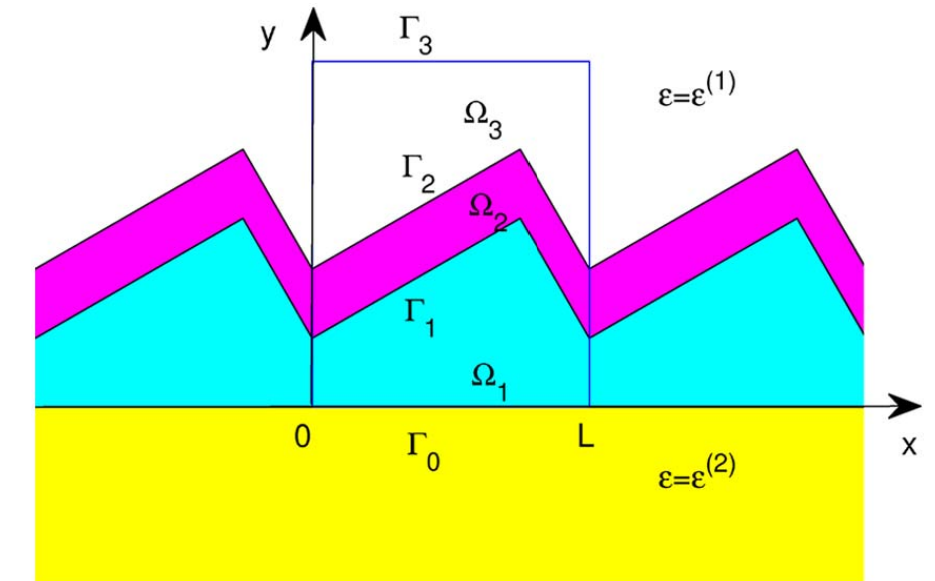
\includegraphics[width=0.6\columnwidth]{figures/diff_grating.png}
\caption{A diffraction grating with multiple layers of different materials. Obtained from \cite{wu2011boundary}.}
\label{fig:diff_grat}
\end{figure}


\section{An overview of existing BIE methods for analyzing diffraction gratings}

Classical BIE formulations for scattering by periodic media rely on the quasi-periodic Green function \cite{linton1998green}. As it is well-known, the standard representation of the quasi-periodic Green function entails evaluating an infinite series that converge slowly and cease to exist at Wood anomalies. Various methods exist to accelerate the convergence of this series, the most notable being Ewald's method \cite{linton1998green}. As a simple alternative, in \cite{monro2008super,bruno2016superalgebraically} the authors utilize a smooth windowed sum approximation of the infinite series, achieving superalgebraically fast convergence away from Wood anomalies.

In another approach developed in \cite{barnett2011new,gillman2013fast}, the quasiperiodic problem is reformulated into a second-kind indirect BIE formulation involving the free-space Green's function and integrating along the infinite boundaries of the unit-cell domain. By exploiting the exponential decay of boundary integrands in spectral form, the resulting BIE system is simplified into a bounded hybrid spatial-spectral computational domain, enabling the application of standard Nyström discretizations for numerical solution. Despite not utilizing the quasi-periodic Green function, this approach requires handling cumbersome Sommerfeld-type integrals, which are particularly challenging in the presence of Wood anomalies, where contour deformations and residue contributions are necessary.

A recent contribution \cite{strauszer2023windowed} follows a similar approach as \cite{barnett2011new,gillman2013fast}: a second-kind indirect
BIE formulation involving the free-space Green’s function is obtained, which requires integrating along the infinite boundaries of the unit-cell domain. However, the infinite boundaries are no longer handled in in the spectral domain, but directly in the spatial domain by relying on the Windowed Green Function (WGF) method \cite{bruno2016windowed} for their computation. 

\textit{This section requires expansion.}

\section{The Boundary Integral Equation Neumann-to-Dirichlet map (BIE-NtD) method}
The BIE-NtD method \cite{wu2009analyzing} is a BIE method for the computation of the reflection and transmission coefficients (\cref{eq:refc,eq:transc}) which relies in (1) the discretization of the boundaries of the retangular domain $\Sigma$ and the material boundaries therein, and (2) the employment of integral operators involving only the free-space Green's function, totally bypassing the use of the quasiperiodic Green's function. The methodology works in a similar fashion as the Transfer Matrix Method (TMM) \cite{born2013principles,heavens1960optical}, which is often employed in the analysis of planar layered and isotropic media: \quote{Transfer Matrices} are constructed for each homogeneous region $\Omega_j$ (see \cref{fig:diff_grat}), which relate the (discretized) values of $u$ and $\partial u/\partial n$ between the boundaries $\Gamma_j$ and $\Gamma_{j+1}$. Then, these Transfer Matrices are concatenated to relate $u$ and $\partial u/\partial n$ of the bottom and top boundaries ($\Gamma_0$ and $\Gamma_3$ in \cref{fig:diff_grat}). With this, the incident wave \cref{eq:incident_wave} and the Rayleigh-Bloch expansions of \cref{eq:refc,eq:transc} can be related, which allows to solve for the reflection and transmission coefficients $R_j$ and $T_j$. The Transfer Matrices are effectively constructed by solving a boundary integral equation and obtaining the NtD map of each homogeneous domain $\Omega_j$.

In this section, instead of presenting a full and technical description of the BIE-NtD method, which can be found in Wu and Lu's paper \cite{wu2009analyzing}, we will present a comparison between the TMM and the BIE-NtD method. In a sense, the BIE-NtD method can be understood as a generalization of the TMM for isotropic layered media with periodic and non-necessarily-planar interfaces.

 Let us start by describing the TMM, employed to analyze reflection and transmission by isotropic layered media. Referring to \cref{fig:t1}, consider the homogeneous region $\Omega_j$ between the planar interfaces $\Gamma_j$ and $\Gamma_{j+1}$, with thickness $h_j$ and permittivity $\epsilon_j$. In the TMM, the values of the $E_z$ and $H_x$ fields between the interfaces $\Gamma_j$ and $\Gamma_{j+1}$ are related by a Transfer Matrix. Since the phase of the wave in the $x$-direction is known and the same for both interfaces (due to continuous translational symmetry in the $x$-direction), then only one discretization point is necessary in each interface to describe the electromagnetic field along the whole interface (the discretization point is marked in purple in \cref{fig:t1}; assume that the $x$-component is the same for both interfaces, say $x=0$). Then, we can write
\begin{align}
\begin{pmatrix}
E_z(y+h_j) \\
H_x(y+h_j) 
\end{pmatrix} 
= M_j
\begin{pmatrix}
E_z(y) \\
H_x(y) 
\end{pmatrix},
\end{align}
where $M_j$ is the Transfer Matrix of region $\Omega_j$. The simplicity of the problem allows us to write $M_j$ in closed form as
\begin{align}
M_j = 
\begin{pmatrix}
\cos(k_jh_j) & iZ_j\sin(k_jh_j) \\
\frac{i}{Z_j}\sin(k_jh_j) & \cos(k_jh_j)
\end{pmatrix},
\end{align}
where $k_j$ is the wavenumber and $Z_j$ is the characteristic impedance of region $\Omega_j$, which depends on $\epsilon_j$ and the angle of incidence. 

\begin{figure}[h!]
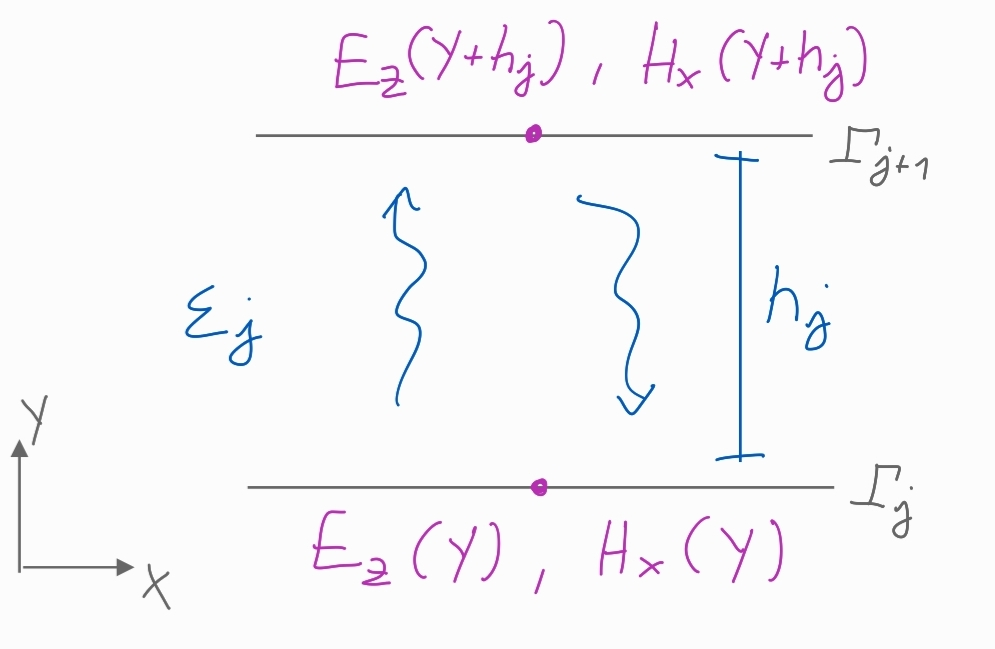
\includegraphics[width=0.6\columnwidth]{figures/t1.jpg}
\caption{An homogeneous region of thickness $h_j$ and permittivity $\epsilon_j$, delimited by the two planar interfaces $\Gamma_j$ and $\Gamma_{j+1}$. The purple point depicts discretization points at the top and bottom interface.}
\label{fig:t1}
\end{figure}

Now, consider a stack of layered regions with total thickness $D$, as shown in \cref{fig:t2}. Given an incident wave from the top, we wish to compute the reflected and transmitted wave generated by this structure. Analogous to what was shown in \cref{sec:problem_form}, we can write the fields in the top and bottom regions as
\begin{align}
E_z^{(\text{top})}(x,y) =& e^{i(\alpha_0 x-\beta_0^{(1)}y)} + Re^{i(\alpha_0 x+\beta_0^{(1)}(y-D))},  \label{eq:tmm_etop}\\
H_x^{(\text{top})}(x,y) =& -\frac{1}{Z_\text{top}}e^{i(\alpha_0 x-\beta_0^{(1)}y)} \nonumber \\&+\frac{1}{Z_\text{top}}Re^{i(\alpha_0 x+\beta_0^{(1)}(y-D))} ,
\end{align}
for $y > D$, and 
\begin{align}
E_z^{(\text{bottom})}(x,y) &= Te^{i(\alpha_0 x-\beta_0^{(2)}y)},  \label{eq:tmm_ebottom}\\
H_x^{(\text{bottom})}(x,y) &= -\frac{1}{Z_\text{bottom}}Te^{i(\alpha_0 x-\beta_0^{(2)}y)} ,
\end{align}
for $y < 0$, where $R$ and $T$ are the reflection and transmission coefficients, respectively. It is convenient, as we shall later see for the BIE-NtD method, to define two Fourier multiplier operators, $\Bcal_\text{TMM}^{(\text{top})}$ and $\Bcal_\text{TMM}^{(\text{bottom})}$, defined by their action on the Fourier basis (or, more precisely, Fourier-Bloch basis):
\begin{align}
i\Bcal_\text{TMM}^{(s)}e^{i\alpha_j x} = \frac{1}{Z_{s}}e^{i\alpha_j x},
\end{align}
for $j\in\Z$ and $s=\text{top}$ or $s=\text{bottom}$. Hence, we can employ these operators to express the magnetic field in terms of the electric field:
\begin{align}
H_x(x,D) &= i\Bcal_\text{TMM}^{(\text{top})}E_z(x,D) - \frac{2}{Z_\text{top}}e^{i\alpha_0 x},\\
H_x(x,0) &= -i\Bcal_\text{TMM}^{(\text{bottom})}E_z(x,0),
\end{align}
for all $x\in\R$. Therefore, following the TMM formalism, we can relate the fields at the top and bottom interface as
\begin{align}
\begin{pmatrix}
E_z(x,D) \\
H_x(x,D) 
\end{pmatrix} 
= M
\begin{pmatrix}
E_z(x,0) \\
H_x(x,0),
\end{pmatrix},
\end{align}
where $M = M_{N-1}M_{N-2}\dots M_1M_0$ is the total Transfer Matrix, obtained by multiplying the Transfer Matrices of each layer. Equivalently, we can write
\begin{align}
\begin{pmatrix}
E_z(x,D) \\
i\Bcal_\text{TMM}^{(\text{top})}E_z(x,D) - \frac{2}{Z_\text{top}}e^{i\alpha_0 x} 
\end{pmatrix} 
\nonumber\\= M
\begin{pmatrix}
E_z(x,0) \\
i\Bcal_\text{TMM}^{(\text{bottom})}E_z(x,0),
\end{pmatrix},
\end{align}
which, for each $x$ (although for this case is sufficient to consider $x=0$ only,) is a linear system of two equations involving two unknowns: $E_z(x,D)$ and $E_z(x,0)$. Once the unknowns are solved, the reflection and transmission coefficients, $R$ and $T$, can be computed from \cref{eq:tmm_etop,eq:tmm_ebottom}, respectively.

\begin{figure}[h!]
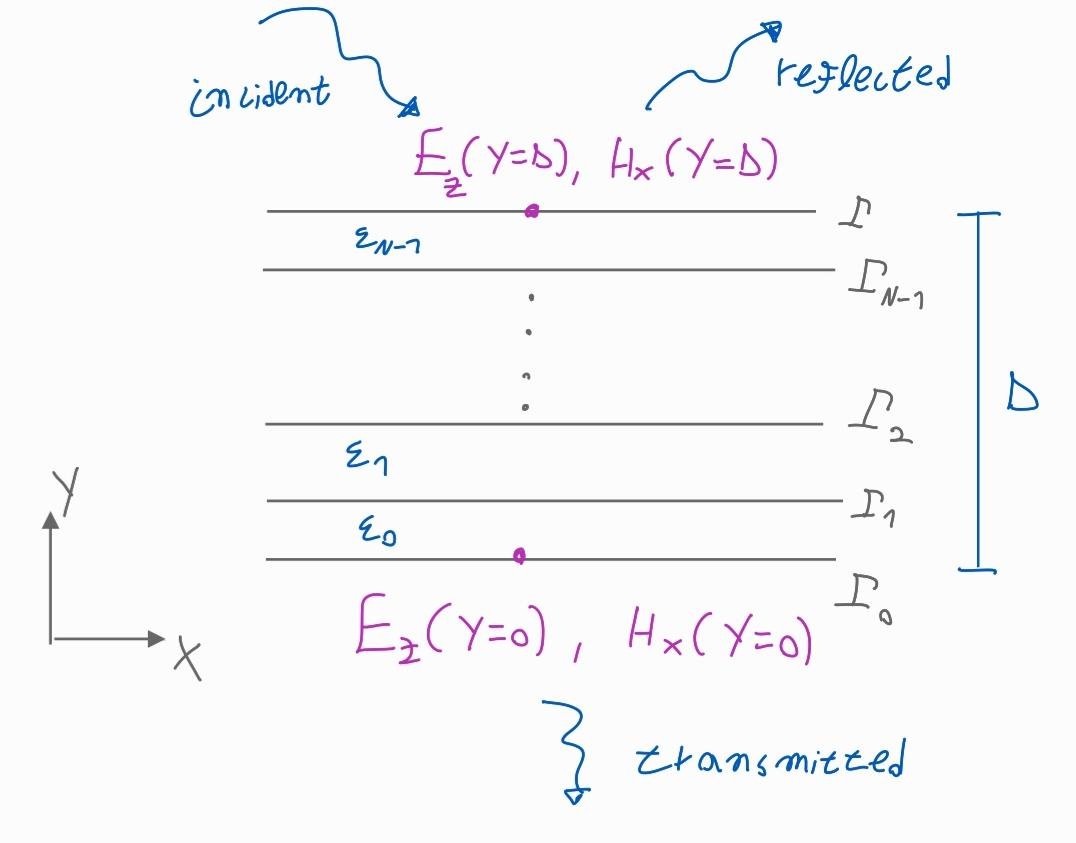
\includegraphics[width=0.6\columnwidth]{figures/t2.jpg}
\caption{A stack of layered regions with planar interfaces and total
thickness D.}
\label{fig:t2}
\end{figure}

The BIE-NtD method, on the other hand, works in exactly the same manner as the TMM; it is, however, much more general, since it allows to handle interfaces that are not necessarily planar, but periodic. 

Consider a region $\Omega_j$, with permittivity $\epsilon_j$, which is delimited by the periodic interfaces $\Gamma_j$ and $\Gamma_{j+1}$, both with period $L$, as depicted in \cref{fig:bie_layer}. The solutions $u$ and $\partial u/\partial n$ at the interfaces can no longer be represented by a single discretization point; in general, they are quasiperiodic functions, with quasiperiod $L$, so an alternative to represent them is to discretize using many points, in only one quasiperiod, along both interfaces $\Gamma_j$ and $\Gamma_{j+1}$, as shown with the purple dots in \cref{fig:bie_layer}. Note that it is not necessary that the $x$-components of the points on the top and bottom interfaces to coincide, or to have the same number of points; moreover, the spacing between points does not have to be uniform. This construction yields four vectors of unknowns, namely $\bol u_{\Gamma_j}$, $ \partial_n \bol u_{\Gamma_j}$, $\bol u_{\Gamma_{j+1}}$, and $ \partial_n \bol u_{\Gamma_{j+1}}$. Now, following the same logic as in the TMM, let us assume that a Transfer Matrix $M_j$ relates the top and bottom unknowns as
\begin{align}
\begin{pmatrix}
\bol u_{\Gamma_{j+1}} \\
\partial_n \bol u_{\Gamma_{j+1}} 
\end{pmatrix} 
= M_j
\begin{pmatrix}
\bol u_{\Gamma_j} \\
\partial_n \bol u_{\Gamma_j} 
\end{pmatrix}.  \label{eq:bie_tmatrix}
\end{align}
For the moment we will assume that $M_j$ exists and it is given. The procedure for its construction will be provided later in \cref{sec:tmatrix}.

\begin{figure}[h!]
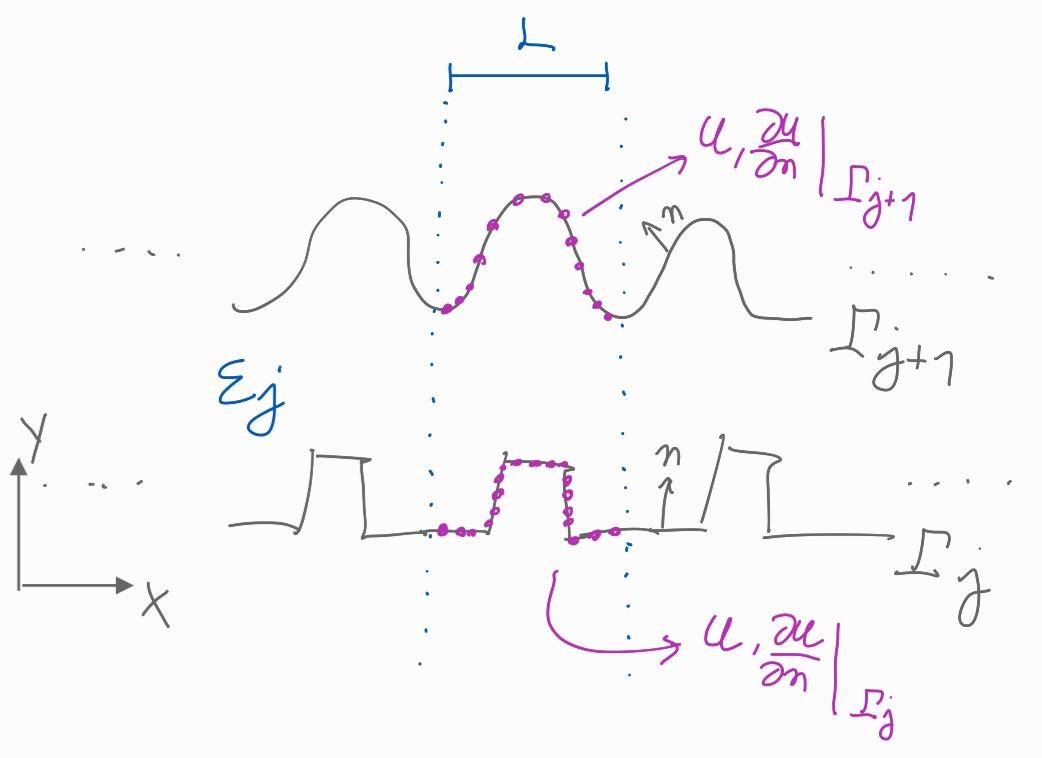
\includegraphics[width=0.6\columnwidth]{figures/bie_layer.jpg}
\caption{An homogeneous region with permittivity $\epsilon_j$, delimited by the two periodic interfaces $\Gamma_j$ and $\Gamma_{j+1}$, with period $L$. The purple points depict discretization points of $u$ and $\partial_n u$ at the top and bottom interface.}
\label{fig:bie_layer}
\end{figure}

Given the Transfer Matrices of all regions, we can consider the diffraction problem (\cref{sec:problem_form}) of a multilayer grating with periodic interfaces, with period $L$, as shown in \cref{fig:bie_multilayer}. The unknowns of the top and bottom interface can be related as
\begin{align}
\begin{pmatrix}
\bol u_{\Gamma_{N}} \\
\partial_n \bol u_{\Gamma_{N}} 
\end{pmatrix} 
= M
\begin{pmatrix}
\bol u_{\Gamma_{0}} \\
\partial_n \bol u_{\Gamma_{0}},
\end{pmatrix}, \label{eq:bie_multilayer_1}
\end{align}
where $M = M_{N-1}M_{N-2}\dots M_1M_0 $ is the total Transfer Matrix, obtained by multiplying the Transfer Matrices of each layer. It is convenient to introduce two Fourier multiplier operators, $\Bcal^{(1)}$ and $\Bcal^{(2)}$, defined by their action on the Fourier basis:
\begin{align}
i\Bcal^{(s)}e^{i\alpha_j x} = i\beta_j^{(s)}e^{i\alpha_j x}, \label{eq:bop}
\end{align}
for $j\in\Z$ and $s=1,2$. In practice, the $i\Bcal^{(s)}$ operators are approximated by matrices; their construction is outlined in \cref{sec:bop}. Hence, using the Rayleigh-Bloch expansions of the top and bottom domains (\cref{eq:refc,eq:transc}) and the fact that the interfaces $\Gamma_N$ and $\Gamma_0$ are flat, and thus $\partial_n = \partial_y$, we can employ $\Bcal^{(1)}$ and $\Bcal^{(2)}$ operators to express $\partial_n \bol u$ in terms of $\bol u$:
\begin{align}
\partial_n \bol u_{\Gamma_{N}}(x) &= i\Bcal^{(1)}\bol u_{\Gamma_{N}}(x) - 2i\beta_0 e^{i\alpha_0 x}, &x \in \Gamma_N,\\
\partial_n \bol u_{\Gamma_{0}}(x) &= -i\Bcal^{(2)}\bol u_{\Gamma_{0}}(x), &x \in \Gamma_0.
\end{align}
Thus, \cref{eq:bie_multilayer_1} can be rewritten as a linear system for two unknowns $\bol u_{\Gamma_{N}}$ and $\bol u_{\Gamma_{0}}$:
\begin{align}
A
\begin{pmatrix}
\bol u_{\Gamma_{N}} \\
\bol u_{\Gamma_{0}} 
\end{pmatrix} 
= \begin{pmatrix}
\bol 0 \\
\bol b
\end{pmatrix} ,
\label{eq:bie_multilayer_2}
\end{align}
where the matrix $A$ is given by, in block matrix form:
\begin{align}
A = 
\begin{pmatrix}
I & -M_{11}+M_{12}i\Bcal^{(2)}\\
i\Bcal^{(1)} & -M_{21}+M_{22}i\Bcal^{(2)}
\end{pmatrix},
\end{align}
where the submatrices $M_{ij}$ are conformable subblocks of the matrix $M$:
\begin{align}
M = 
\begin{pmatrix}
M_{11} & M_{12}\\
M_{21} & M_{22}
\end{pmatrix},
\end{align}
and the vector $\bol b$ is given by $\bol b = (2i\beta_0 e^{i\alpha_0 x} \text{ for } x \in \Gamma_N)^\top$. Solving \cref{eq:bie_multilayer_2} yields $\bol u_{\Gamma_{N}}$ and $\bol u_{\Gamma_{0}}$. To obtain the reflection and transmission coefficients, we notice that the reflected field at $\Gamma_N$, given by $\bol u^{(r)} = \bol u_{\Gamma_{N}}-\bol u_{\Gamma_{N}}^{(i)}$, and the transmitted field at $\Gamma_0$, which is $\bol u^{(t)} = \bol u_{\Gamma_{0}}$, can be written using \cref{eq:refc,eq:transc} as
\begin{align}
u^{(r)}(x) =& \sum\limits_{j=-\infty}^\infty R_je^{i\alpha_jx }, &x \in \Gamma_N,\\
u^{(t)}(x) =& \sum\limits_{j=-\infty}^\infty T_je^{i\alpha_jx}, &x \in \Gamma_0.
\end{align}
Thus, the reflection ans transmission coefficients can be obtained by inverting these Fourier-Bloch series:
\begin{align}
    R_j &= \frac{1}{L}\int_0^L u^{(r)}(x)e^{-i\alpha_jx}\de x,\\
    T_j &= \frac{1}{L}\int_0^L u^{(t)}(x)e^{-i\alpha_jx}\de x,\\
\end{align}
for $j \in \Z$, which can be computed numerically by employing the discretizations $\bol u^{(r)}$ and $\bol u^{(t)}$.

\begin{figure}[h!]
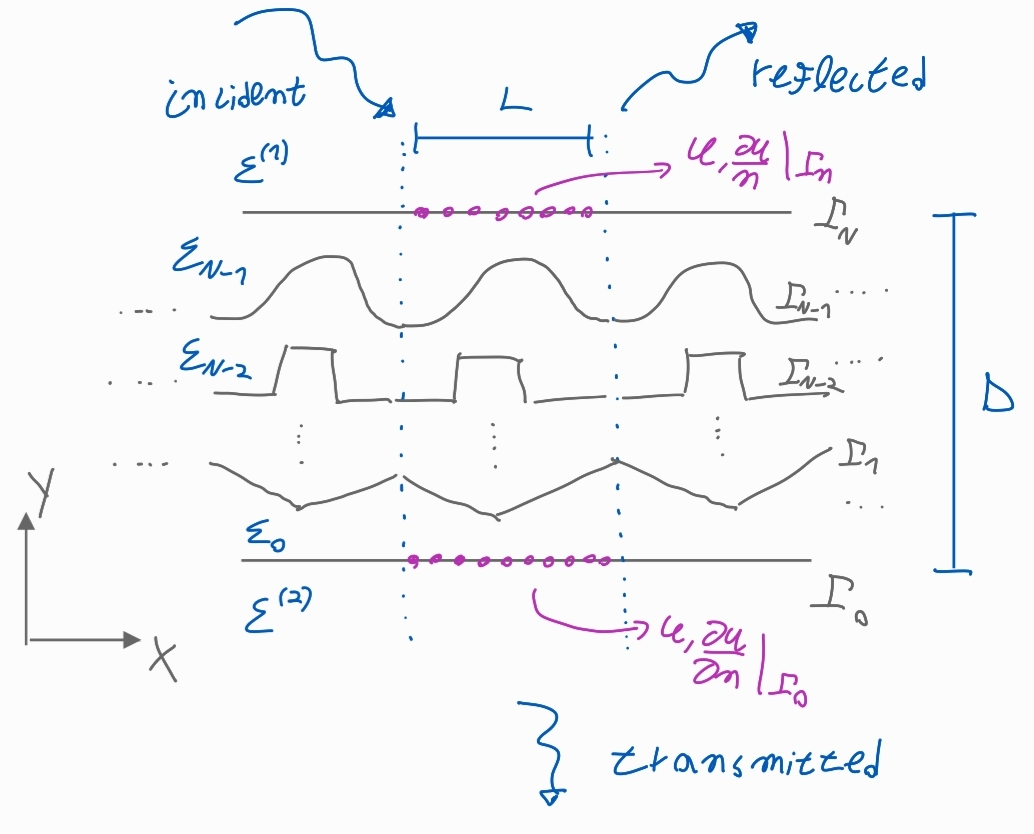
\includegraphics[width=0.6\columnwidth]{figures/bie_multilayer.jpg}
\caption{A stack of layered regions with periodic interfaces, with period $L$,
and total thickness D.}
\label{fig:bie_multilayer}
\end{figure}

\subsection{Construction of the Transfer Matrix via the NtD map}\label{sec:tmatrix}
A key component of the BIE-NtD method is the construction of the Transfer Matrices $M_j$, which relate the values of $u$ and $\partial_n u$ between two adjacent interfaces, as shown in \cref{eq:bie_tmatrix}, and, as the name of the method implies, their construction involves solving a Boundary Integral Equation and computing the Neumann-to-Dirichlet map of each homogeneous region.

In a closed region $\Omega_j$, with boundary $\partial\Omega_j$ and normal vector $\bol n$ pointing outwards, the Neumann-to-Dirichlet map is an operator that relates the values of $u$ and $\partial_n u$ on the boundary $\partial\Omega_j$, a relation that can be written as 
\begin{align}
    \bol u_{\partial\Omega_j} = \Vcal_j \lf(\partial_n \bol u_{\partial\Omega_j}\rg), \label{eq:ntd1}
\end{align}
where $\Vcal_j$ is the NtD map of region $\Omega_j$. In practice, $\Vcal_j$ is approximated by a matrix that relates the point values of $u$ and $\partial_n u$ on the boundary; its construction is outlined in \cref{sec:ntdmap}. 

Consider, for instance, a closed domain $\Omega_j$, with permittivity $\epsilon_j$, delimited by the interfaces $\Gamma_j$ and $\Gamma_{j+1}$, and by vertical boundaries at $x=0$ and $x=L$, as illustrated in \cref{fig:bie_domain}. Denoting $\bol v_j = \bol u\rvert_{x=0}$, $\bol w_j = \bol u\rvert_{x=L}$, $\bol u_j = \bol u\rvert_{\Gamma_j}$, and $\bol u_{j+1} = \bol u\rvert_{\Gamma_{j+1}}$, we can rewrite \cref{eq:ntd1} by partitioning $\Vcal_j$ in blocks:
\begin{align}
\begin{pmatrix}
    \bol u_{j-1}\\
    \bol v_j\\
    \bol w_j\\
    \bol u_{j}
\end{pmatrix}
= 
\begin{pmatrix}
    \Vcal_{11} & \Vcal_{12} & \Vcal_{13} & \Vcal_{14}\\
    \Vcal_{21} & \Vcal_{22} & \Vcal_{23} & \Vcal_{24}\\
    \Vcal_{31} & \Vcal_{32} & \Vcal_{33} & \Vcal_{34}\\
    \Vcal_{41} & \Vcal_{42} & \Vcal_{43} & \Vcal_{44}
\end{pmatrix}
\begin{pmatrix}
    \partial_n \bol u_{j-1}\\
    \partial_n \bol v_j\\
    \partial_n \bol w_j\\
    \partial_n \bol u_{j}
\end{pmatrix}.
\label{eq:ntd2}
\end{align}
Our goal is to relate $(\bol u_{j+1}, \partial_n \bol u_{j+1})$ with $(\bol u_{j}, \partial_n \bol u_{j})$ using a Transfer Matrix $M_j$. If $(\bol u_{j}, \partial_n \bol u_{j})$ are given, then \cref{eq:ntd2} is a linear system of $4r$ equations, where $r$ is the length of each vector, for $6r$ unknowns, which are $\bol u_{j+1}, \partial_n\bol u_{j+1},\bol v_j, \partial_n\bol v_j,\bol w_j$, and  $\partial_n\bol w_j$. (For simplicity we have assumed that each vector has the same length $r$; however, this argument still works if we only demand that the lateral unknowns $\bol v_j, \partial_n\bol v_j,\bol w_j, \partial_n\bol w_j$ have the same length.)
Notice that the Bloch-periodic boundary conditions of \cref{eq:bloch1,eq:bloch2} provide us with additional $2r$ equations, namely
\begin{align}
    \bol w_j &= \gamma \bol v_j, \label{eq:bloch_ntd1}\\
    \partial_n \bol w_j &= -\gamma \partial_n \bol v_j, \label{eq:bloch_ntd2}
\end{align}
and thus we have a square system for our $6r$ unknowns. To obtain the Transfer Matrix $M_j$, we can formally express the lateral unknowns in terms of $\bol u_{j+1}$ and $\partial_n\bol u_{j+1}$, and then eliminate them from the system of equations (this is done via \textit{Schur complements}), after which we finally obtain a system of equations that relates $(\bol u_{j+1},\partial_n\bol u_{j+1})$ with $(\bol u_{j},\partial_n\bol u_{j})$, this is 
\begin{align}
\begin{pmatrix}
\bol u_{j+1} \\
\partial_n \bol u_{j+1} 
\end{pmatrix} 
= M_j
\begin{pmatrix}
\bol u_{j} \\
\partial_n \bol u_{j} 
\end{pmatrix},
\end{align}
where the Transfer Matrix $M_j$ was obtained by eliminating the lateral variables from \cref{eq:ntd2,eq:bloch_ntd1,eq:bloch_ntd2}.

\begin{figure}[h!]
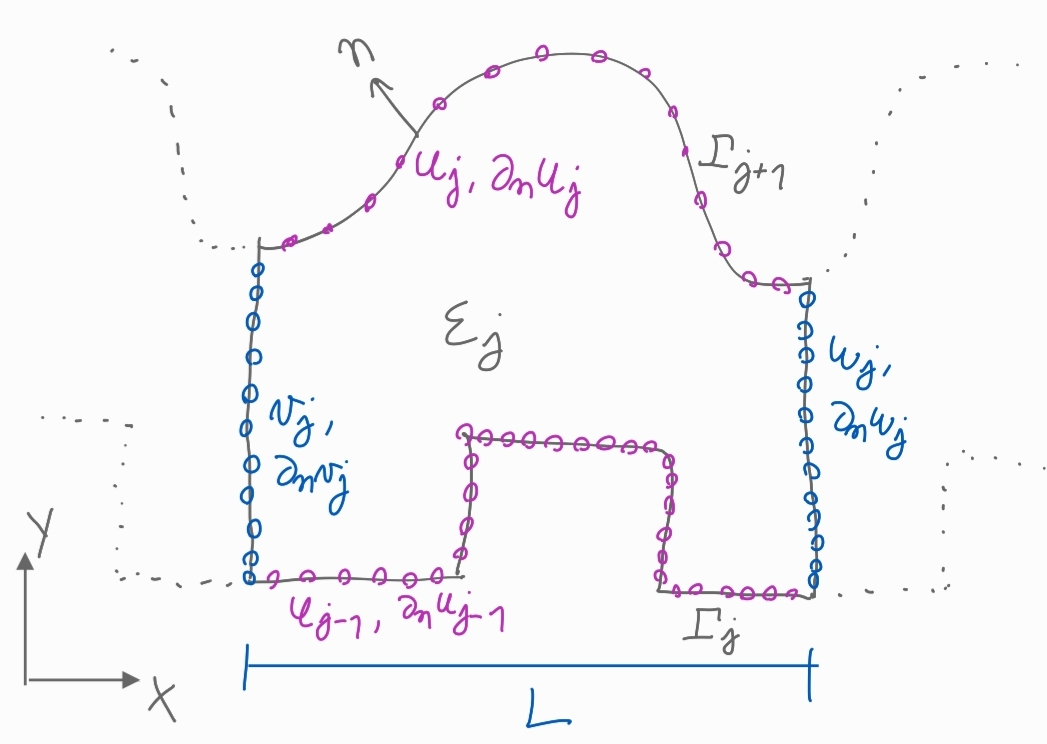
\includegraphics[width=0.6\columnwidth]{figures/bie_domain.jpg}
\caption{A closed region with permittivity $\epsilon_j$, delimited by the two periodic interfaces $\Gamma_j$ and $\Gamma_{j+1}$, with period $L$, and vertical walls at $x=0$ and $x=L$. The purple and blue points depict discretization points of $u$ and $\partial_n u$ at the boundary of the domain.}
\label{fig:bie_domain}
\end{figure}

\subsection{Construction of the NtD map}\label{sec:ntdmap}
A way of constructing the NtD map for a closed region is to rely on \textit{the Green's representation formula} \cite{colton2013integral}, also known as \textit{the Principle of Equivalence}, which asserts that a solution $u$ of the Hemlholtz equation in a closed domain $\Omega$ can be express solely in terms of the values of $u$ and $\partial_n u$ on the boundary $\Gamma = \partial\Omega$. For a closed domain $\Omega$ with wavenumber $k$, such as the one shown in \cref{fig:bie_domain} (for simplicity let us drop the subscripts $j$,) we have that 
\begin{align}
    u(x) = \Scal[\partial_n u](x) - \Dcal[u](x), \qquad x\in \Omega,
\end{align}
where 
\begin{align}
    \Scal[\phi](x) &= \oint_{\Gamma}G(x,y)\phi(y)\de s_y,\\
    \Dcal[\phi](x) &= \oint_{\Gamma}\frac{\partial G(x,y)}{\partial_{n_y}}\phi(y)\de s_y, \quad x\in \Omega,
\end{align}
are the \textit{single-layer} and \textit{double-layer} potentials, $G(x,y) = \tfrac{i}{4}H_0^{(1)}(k \abs{x-y})$ is the \textit{free-space Green's function} of the Helmholtz equation in two dimensions, and $H_0^{(1)}$ is the Hankel function of the first kind of order zero.
By taking the limit $x\rightarrow \Gamma$, and taking into account the well-known jump of the double-layer potential \cite{colton2013integral}, we have that
\begin{align}
    \frac{u(x)}{2}+\Dcal[u](x) = \Scal[\partial_n u](x), \qquad x\in \Gamma,
\end{align}
or in its discretized form,
\begin{align}
    \left(\frac{I}{2} + \mathrm{D}\right)\bol u_{\Gamma} = \mathrm{S}(\partial_n \bol u_{\partial\Omega}), \label{eq:bie_fredh}
\end{align}
which is a Fredholm integral equation of the second kind for $\bol u_{\Gamma}$. Then, we have that
\begin{align}
    \bol u_{\Gamma} = \left(\frac{I}{2} + \mathrm{D}\right)^{-1}\mathrm{S}(\partial_n \bol u_{\Gamma}),
\end{align}
and thus the Neumann-to-Dirichlet map is given by $\Vcal = \left(\tfrac{I}{2} + \mathrm{D}\right)^{-1}\mathrm{S}$. The inverse of the $\left(\tfrac{I}{2} + \Dcal\right)$ operator always exists, except for a discrete and infinite set of $k^2$ wavenumbers that correspond to the Neumann eigenvalues of the domain $\Omega$ \cite{colton2013integral}.

\subsection{Construction of the $i\Bcal^{(1)}$ and $i\Bcal^{(2)}$ operators}\label{sec:bop}
Consider a quasiperiodic function $f$ with quasiperiod $L$, which can be written as a Fourier-Bloch series:
\begin{align}
    f(x) = \sum\limits_{j=-\infty}^\infty \hat{f}_je^{i\alpha_jx}, \quad x \in [0,L],
\end{align}
where 
\begin{align}
    \hat{f}_j &= \frac{1}{L}\int_0^L f(x)e^{-i\alpha_jx}\de x, \quad j\in\Z.
\end{align}
By definition, we have that (\cref{eq:bop})
\begin{align}
    (i\Bcal^{(s)}f)(x) = \sum\limits_{j=-\infty}^\infty i\beta^{(s)}\hat{f}_je^{i\alpha_jx}, \quad x \in [0,L],
\end{align}
for $s = 1,2$. Therefore,
\begin{align}
    (i\Bcal^{(s)}f)(x) = \sum\limits_{j=-\infty}^\infty i\beta^{(s)}\left(\frac{1}{L}\int_0^L f(t)e^{-i\alpha_jt}\de t\right)e^{i\alpha_jx}
\end{align}
for $x \in [0,L]$, which can be numerically computed using the point values of $f$ along $[0,L]$.

\subsection{Regions with inclusions}
The BIE-NtD method is also compatible with regions with inclusions; the only difference is that the NtD map $\Vcal$ must be slightly modified. Consider the region with inclusion shown in \cref{fig:bie_inclusion}, which consists in an interior region, with wavenumber $k_B$ and boundary $\Gamma_B$, embedded in an exterior region with wavenumber $k_A$ and boundary $\Gamma_A$. Denote by $\mathrm{S}_{AB}$ the matrix that maps a density $\phi_B$, defined on $\Gamma_B$, onto $\Gamma_A$ using the single-layer operator, and similarly for $\mathrm{S}_{BA}$ and the double-layer operator (all operators use the same $k_A$ wavenumber). Then, similarly as \cref{eq:bie_fredh}, we have
\begin{align}
    \frac{\bol u_A}{2} = \mathrm{S}_{AA}(\partial_n \bol u_A) - \mathrm{D}_{AA}\bol u_A - \mathrm{S}_{AB}(\partial_n \bol u_B) - \mathrm{D}_{AB}\bol u_B,\\
    \frac{\bol u_B}{2} = \mathrm{S}_{BA}(\partial_n \bol u_A) - \mathrm{D}_{BA}\bol u_A - \mathrm{S}_{BB}(\partial_n \bol u_B) - \mathrm{D}_{BB}\bol u_B,
\end{align}
where $\bol u_A$ denotes the values of $u$ on $\Gamma_A$, and similarly for $\bol u_B$. Using the NtD map $\Vcal_B$ of the interior region, we have that $\bol u_B=\Vcal_B(\partial_n \bol u_B)$, and thus, after some tedious algebra, we can eliminate $\bol u_B$ and $\partial_n \bol u_B$ from the previous equations to yield a modified NtD map $\tilde{\Vcal}$ such that
\begin{align}
    u_A=\tilde{\Vcal}_A(\partial_n \bol u_A).
\end{align}

\begin{figure}[h!]
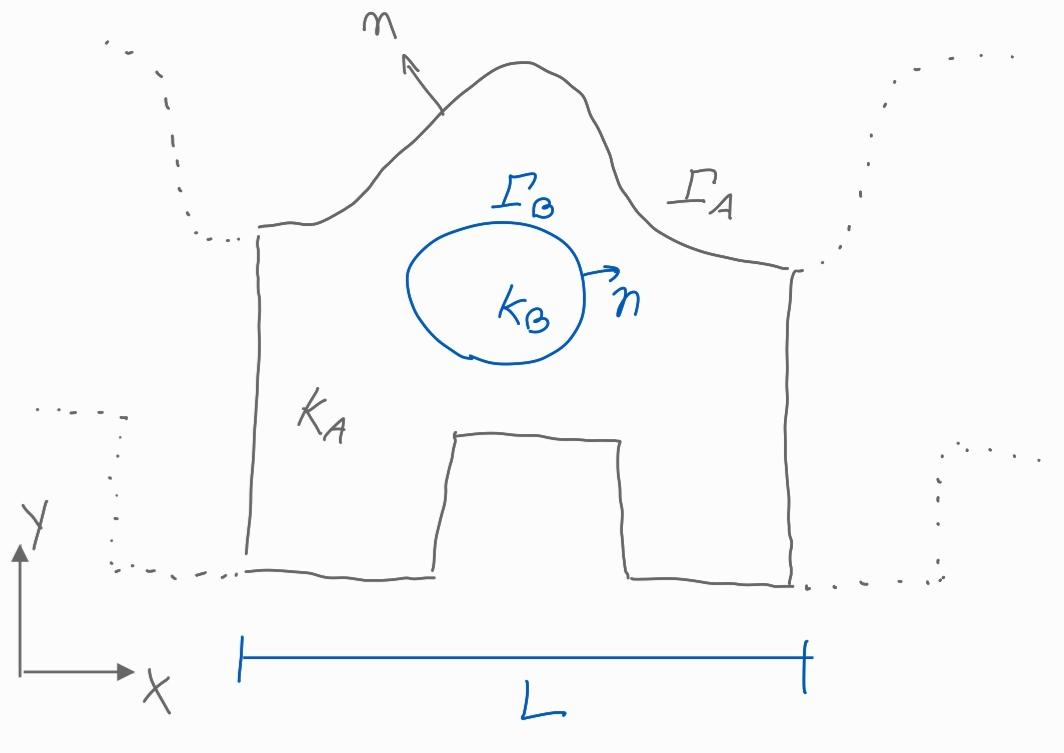
\includegraphics[width=0.6\columnwidth]{figures/bie_inclusion.jpg}
\caption{Region with inclusion. An interior region, with wavenumber $k_B$ and boundary $\Gamma_B$, is embedded in an exterior region with wavenumber $k_A$ and boundary $\Gamma_A$.}
\label{fig:bie_inclusion}
\end{figure}


\section{Numerical examples}
The BIE-NtD method was programmed in the Julia Programming Language. Non-singular integral operators were discretized using the trapezoidal rule, whereas singular integral operators were discretized using the spectrally-accurate Nyström method by Martensen and Kussmaul \cite{martensen1963methode,kussmaul1969numerisches}, as described by Colton and Kress \cite{colton1998inverse}. As suggested by the latter authors, and by Wu and Lu \cite{wu2009analyzing}, we employed a graded mesh to resolve possible singularities of the integral densities at the domains' corners. The code is available at \url{https://github.com/Riarrieta/DiffGrating1D}.

\subsection{First example}
For our first numerical example, which serves as a validation of our code, we consider the two sinusoidal gratings of \cref{fig:ex1}. The first one comprises a sinusoidal profile which separates air and a different homogeneous medium. For a grove depth of $d=L$, a wavelength of $\lambda=L/1.7$ and $\alpha_0 = \pi/\lambda$, the computed reflection and transmission efficiencies are shown in \cref{tab:ex1}, where we also compare our values with the ones obtained by Li \cite{li1993multilayer}, employing the C method, and by Wu and Lu \cite{wu2009analyzing}. Using a similar discretization as Wu an Lu, it is observed that our results match their results, at least up to six decimal places. For the second grating with parameters $d_1 = 0.1L/\pi$, $d_2 = 0.4L/\pi$, which has a limited extent in the $y$-direction and separates two regions of air, we considered two different incident plane waves: one with $\lambda = L/1.9$ and angle of incidence of $15.2575^\circ$, measured with respect to the $y$-axis, and another with $\lambda = L$ and angle of incidence of $30^\circ$. For each case we compared our computed reflection and transmission efficiencies with results obtained by Magath et al. \cite{magath2005fast} and by Wu and Lu \cite{wu2009analyzing}; this is shown in \cref{tab:ex1_2}. It is observed that our results, obtained with a similar discretization as the one used by Wu and Lu, match the results of the other authors, up to five decimal places. 

\begin{figure}[h!]
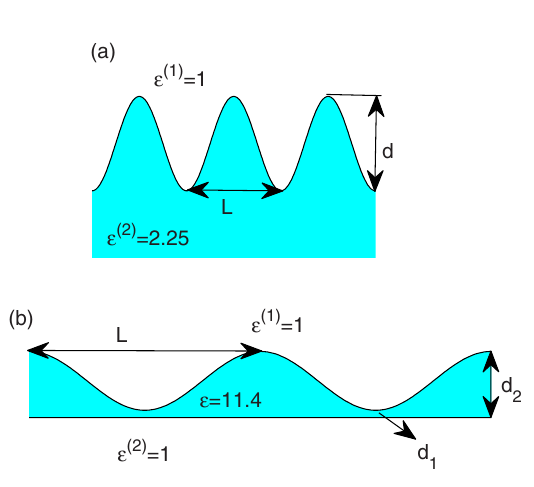
\includegraphics[width=0.6\columnwidth]{figures/ex1.png}
\caption{Two sinusoidal diffraction gratings. In (a) the sinusoidal profile divides air and an homogeneous region. In (b) the grating has finite thickness and divides two regions of air.}
\label{fig:ex1}
\end{figure}

\begin{table}[h!]
\centering
\caption{First example. Reflection and transmission efficiencies for various diffraction orders, for grating (a) of \cref{fig:ex1}.}    
\begin{ruledtabular}
\begin{tabular}{clll}
Order & \multicolumn{1}{c}{Li \cite{li1993multilayer}}    & \multicolumn{1}{c}{Wu and Lu \cite{wu2009analyzing}} & \multicolumn{1}{c}{This work} \\ \hline
R, -1 & $0.7815037\times 10^{-3}$ & $0.78150378\times 10^{-3}$    & $0.78150394\times 10^{-3}$    \\
R, 0  & $0.2103160\times 10^{-2}$ & $0.21031606\times 10^{-2}$    & $0.21031607\times 10^{-2}$    \\
T, -1 & 0.4947933                 & 0.49479330                    & 0.49479329                    \\
T, 0  & 0.2086662                 & 0.20866625                    & 0.20866625                    \\
T, 1  & 0.1183058                 & 0.11830582                    & 0.11830581                   
\end{tabular}          
\end{ruledtabular}
\label{tab:ex1}
\end{table}

\begin{table}[h!]
\centering
\caption{Second example. Reflection and transmission efficiencies for various diffraction orders, for grating (b) of \cref{fig:ex1}.}
\label{tab:ex1_2} 
\begin{ruledtabular}
\begin{tabular}{cclll}
\multicolumn{1}{l}{$L/\lambda$} & Order                     & \multicolumn{1}{c}{Magath et al. \cite{magath2005fast}} & \multicolumn{1}{c}{Wu and Lu} \cite{wu2009analyzing} & \multicolumn{1}{c}{This work} \\ \hline
1.9                             & R, -2                     & 0.1632                            & 0.16337787                    & 0.16337768                    \\
1.9                             & R, -1                     & 0.5312                            & 0.53111858                    & 0.53111788                    \\
1.9                             & R, 0                      & 0.0650                            & 0.06506795                    & 0.06506801                    \\
1.9                             & R, 1                      & 0.1538                            & 0.15381827                    & 0.15381866                    \\ \hline
1                               & R, -1                     & 0.0401                            & 0.03989897                    & 0.03989898                    \\
1                               & \multicolumn{1}{l}{R, 0}  & 0.4777                            & 0.47833249                    & 0.47833248                    \\
1                               & \multicolumn{1}{l}{T, -1} & 0.2794                            & 0.27947198                    & 0.27947200                    \\
1                               & \multicolumn{1}{l}{T, 0}  & 0.2029                            & 0.20229650                    & 0.20229652                   
\end{tabular} 
\end{ruledtabular}
\end{table}

\subsection{Second example}
We consider the second grating of \cref{fig:ex1}, but with a variable sinusoidal amplitude, given by $A\times 0.4L/\pi$ (originally $A=1$.) For $A=0.5$ we plotted the transmission efficiency of the zeroth-order as a function of angular frequency $\omega$ and Bloch wavevector $\alpha_0$ ($k_x$ in the figures), which is shown in \cref{fig:ex4_w_kx_T}. We observe clear zig-zagging dips in the transmittance spectrum, which correspond to guided modes of the structure that become leaky as the periodic sinusoidal profile is introduced. These leaky modes give rise to a characteristic Fano resonance lineshape \cite{fan2003temporal}, which can be observed in \cref{fig:ex4_w_singlekx_T}, where the transmission efficiency as a function of angular frequency is plotted, for $\alpha_0 L / 2\pi = 0.245$. Here, a strange kink around $\omega L / 2\pi c = 0.75$ can be observed, which can also be noted at the top left corner of \cref{fig:ex4_w_kx_T_v1}; its origin is unknown.

\begin{figure}[h!]
\begin{subfigure}{.5\textwidth}
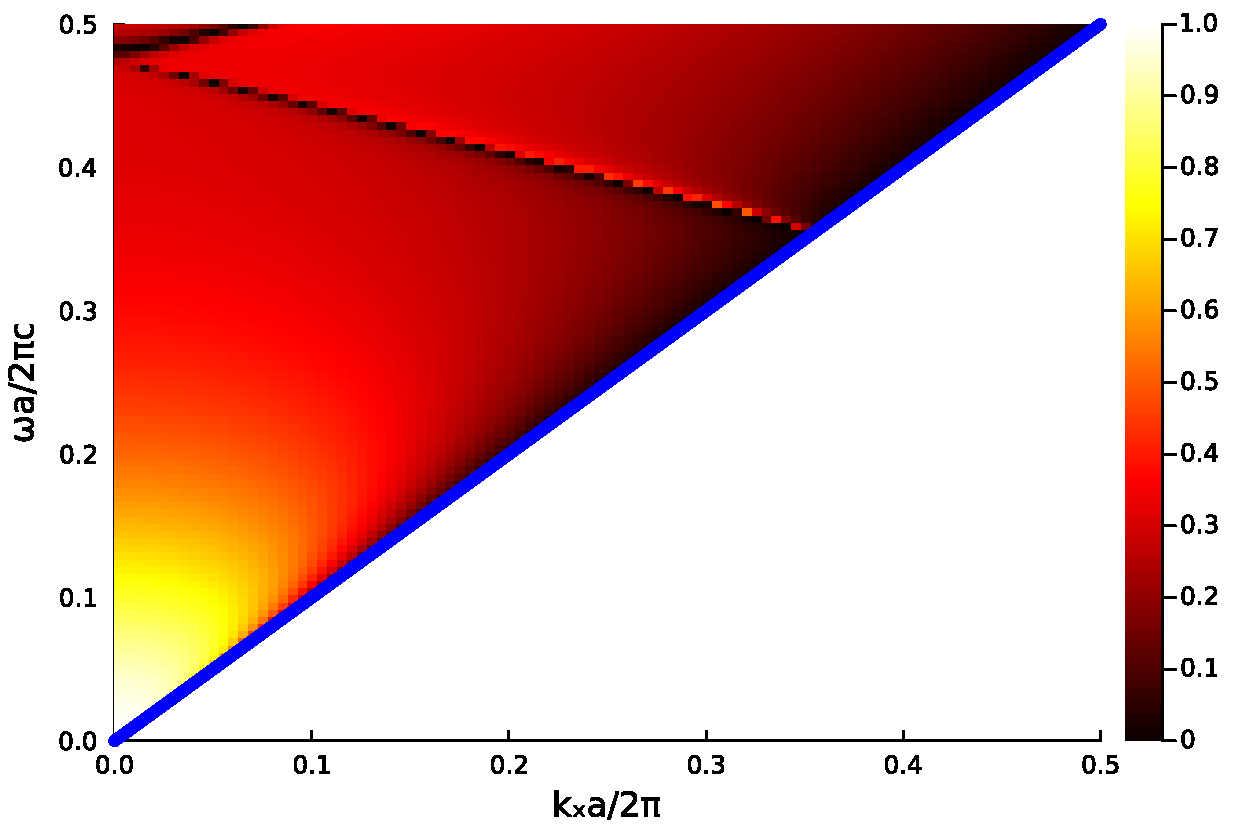
\includegraphics[width=0.6\columnwidth]{figures/ex4_w_kx_T_v2.pdf}
  \caption{Transmittance for normalized angular frequency between $0$ and $0.5$. The light line is shown in blue.}
\label{fig:ex4_w_kx_T_v2}
\end{subfigure}
\begin{subfigure}{.5\textwidth}
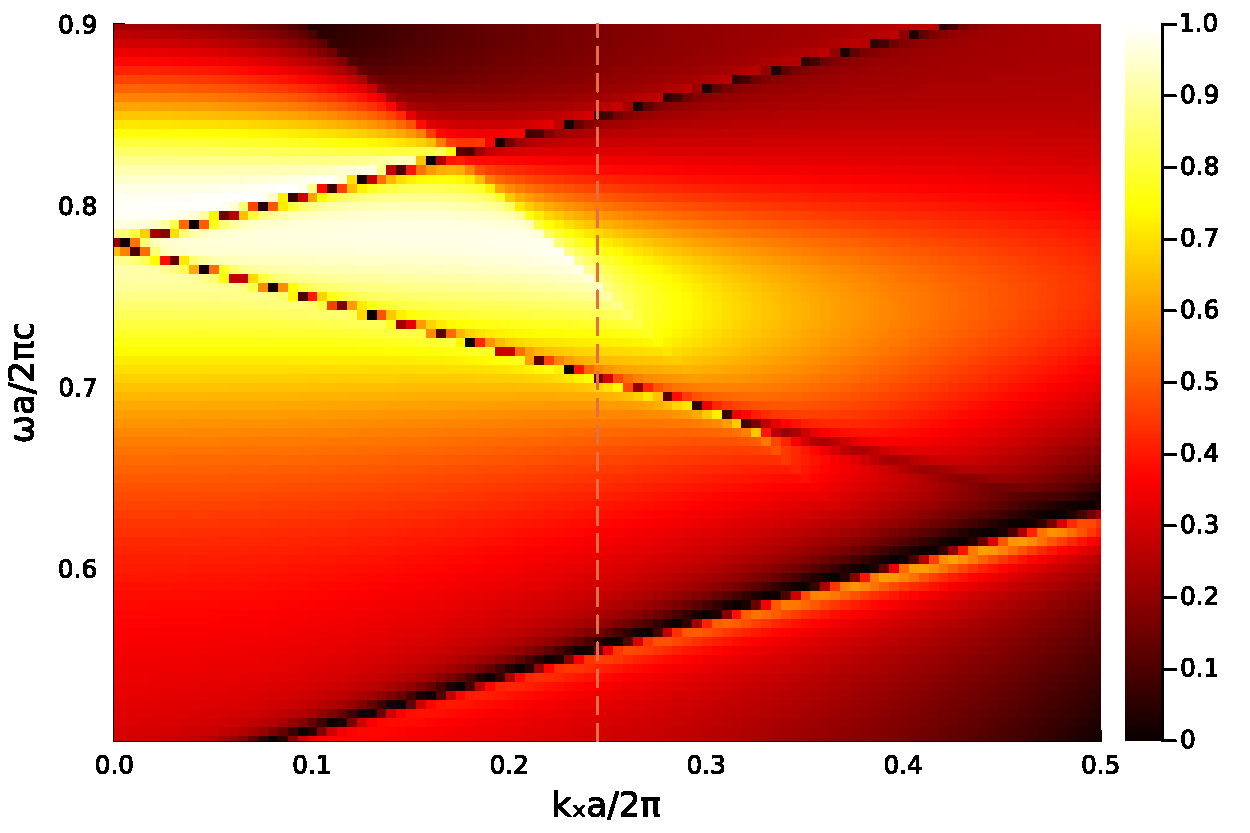
\includegraphics[width=0.6\columnwidth]{figures/ex4_w_kx_T_v1.pdf}
  \caption{Transmittance for normalized angular frequency between $0.5$ and $0.9$. We mark the normalized Bloch wavenumber $0.25$ with a dashed line. The transmittance for this value is later plotted in \cref{fig:ex4_w_singlekx_T}.}
\label{fig:ex4_w_kx_T_v1}
\end{subfigure}
\caption{Second example. Transmittance of the zeroth-order diffraction as a function of angular frequency and Bloch wavenumber.}
\label{fig:ex4_w_kx_T}
\end{figure}

\begin{figure}[h!]
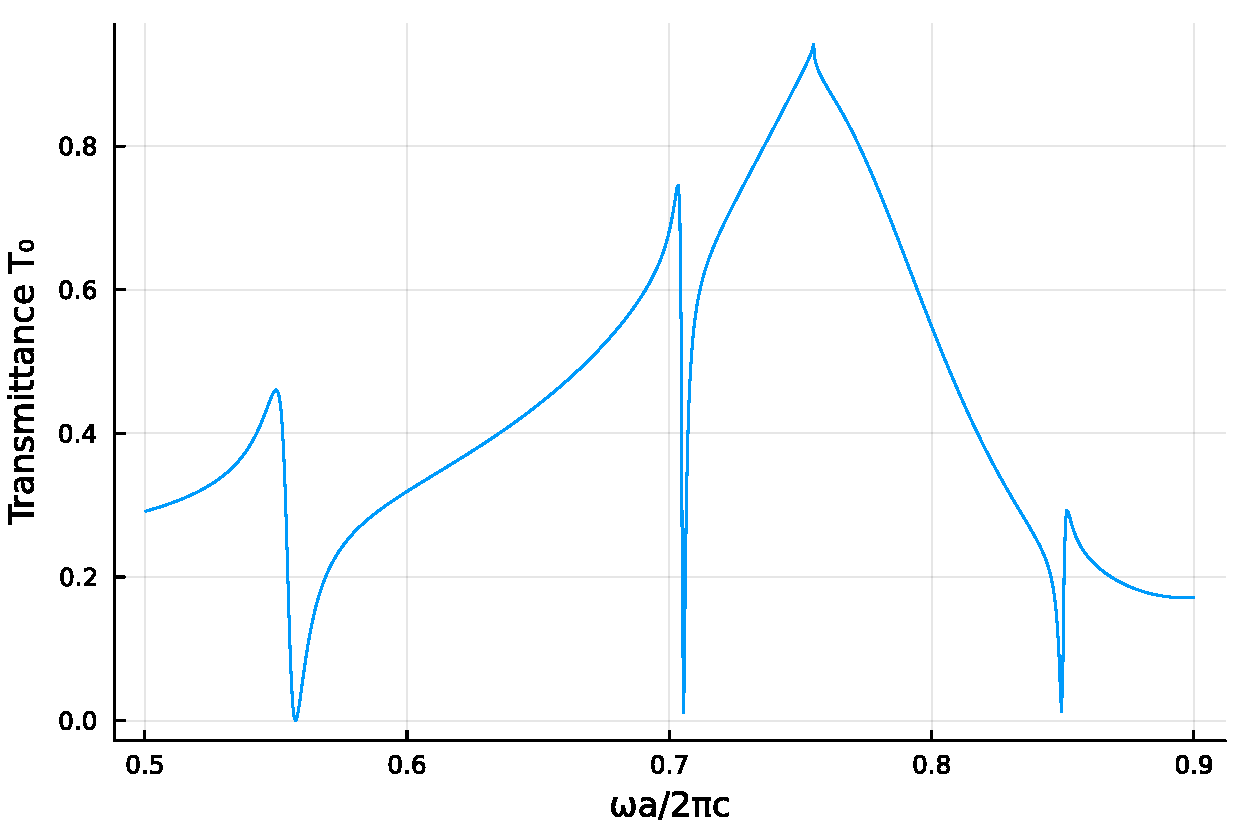
\includegraphics[width=0.6\columnwidth]{figures/ex4_w_singlekx_T.pdf}
\caption{Second example. Transmittance as a function of normalized angular frequency, for a normalized Bloch wavenumber of 0.25, as marked with a dashed line in \cref{fig:ex4_w_kx_T_v1}.}
\label{fig:ex4_w_singlekx_T}
\end{figure}

\subsection{Third example}
We consider again the second grating of \cref{fig:ex1} with a variable sinusoidal amplitude of $A\times 0.4L/\pi$. For normal incidence ($\alpha_0 = 0$) we plotted the transmission efficiency of the zeroth-order as a function of angular frequency $\omega$, for three values of the amplitude $A$: $0$, $0.01$ and $0.1$. This is shown in \cref{fig:ex4_fano}. As expected, for $A=0$ the transmittance spectrum follows a typical Fabry–Pérot spectrum. However, for $A>0$ we have that a previously guided mode becomes leaky and couples with external radiation, giving rise to a typical Fano lineshape around $\omega L /2\pi c \approx 0.995$, whose width increases as we increase the amplitude $A$.

\begin{figure}[h!]
\begin{subfigure}{.5\textwidth}
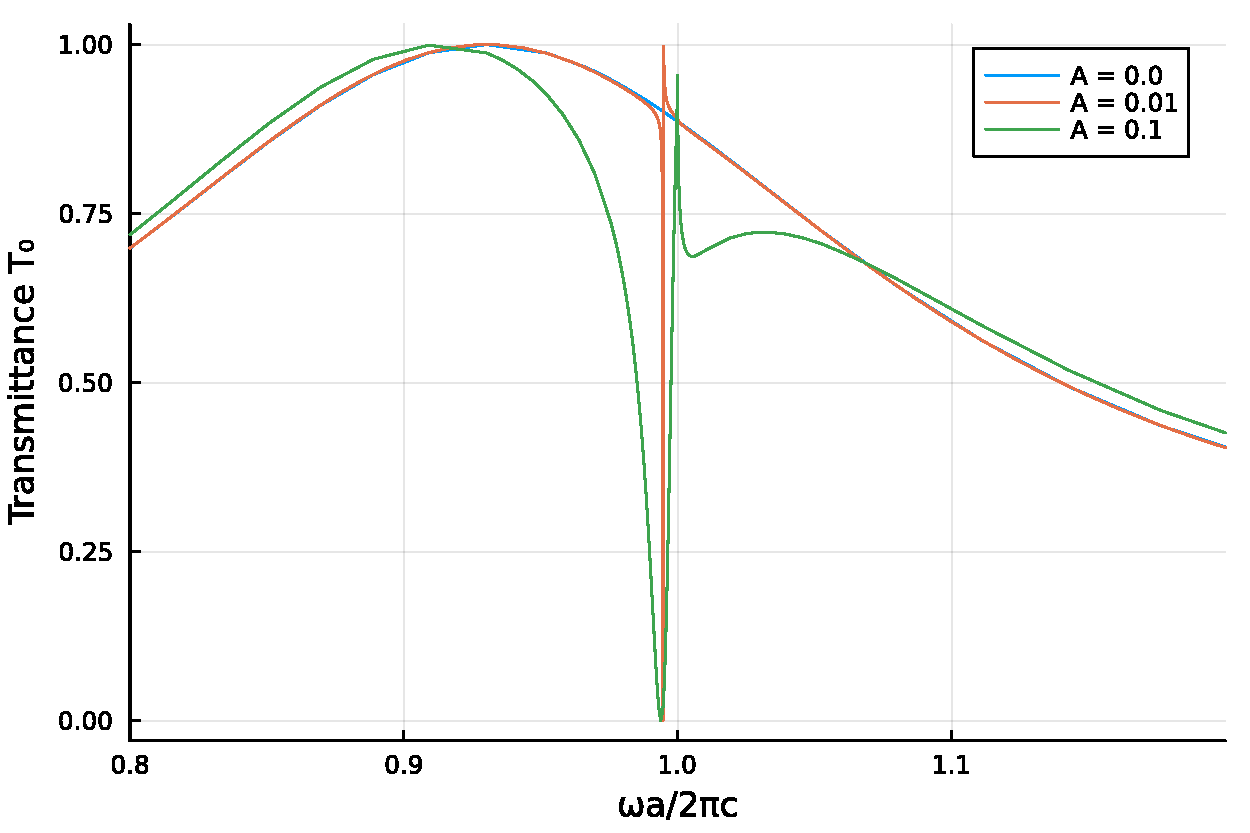
\includegraphics[width=0.6\columnwidth]{figures/ex4_fano_v1.pdf}
  \caption{Normalized angular frequency between 0.8 and 0.2.}
\label{fig:ex4_fano_v1}
\end{subfigure}
\begin{subfigure}{.5\textwidth}
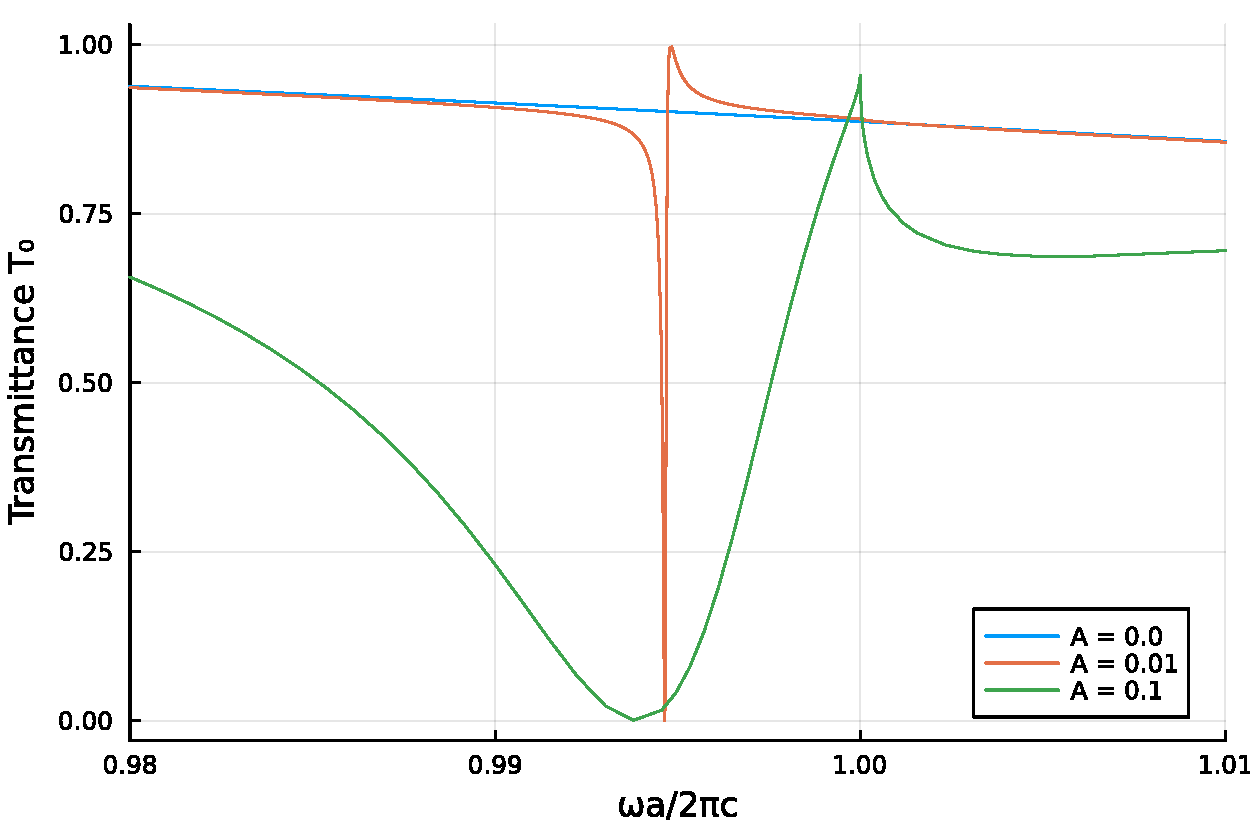
\includegraphics[width=0.6\columnwidth]{figures/ex4_fano_v2.pdf}
  \caption{Normalized angular frequency between 0.98 and 1.01.}
\label{fig:ex4_fano_v2}
\end{subfigure}
\caption{Third example. Transmittance of the zeroth-order diffraction as a function of normalized angular frequency, for various values of the sinusoidal amplitude $A$. A Fano lineshape is clearly distinguishable.}
\label{fig:ex4_fano}
\end{figure}

\subsection{Fourth example}
We consider again the second grating of \cref{fig:ex1} with a variable sinusoidal amplitude of $A\times 0.4L/\pi$, but this time adding a second harmonic to the profile, with amplitude $B\times 0.4L/\pi$ and phase $\phi = \pi/15$, which, for $B > 0$, breaks the mirror symmetry with respect to the $yz$ plane. In \cref{fig:ex4_bic}, for normal incidence light ($\alpha_0 = 0$), we plot the transmission efficiency of the zeroth-order as a function of angular frequency $\omega$, for various values of $A$ and $B$. As expected, for $A=0$ the transmittance spectrum follows a typical Fabry–Pérot spectrum, whereas for $A>0$ a Fano lineshape emerges at $\omega L /2\pi c \approx 0.995.$ What it is interesting is that for $A > 0$ and $B>0$ a second Fano lineshape emerges at $\omega L /2\pi c \approx 0.772$. We hypothesize that, at $B=0$, a Bound State in the Continuum (BiC) \cite{hsu2016bound} is found around $\omega L /2\pi c \approx 0.772$. This is a guided mode, which is present in the radiative spectrum, but does not couple to it, it thus remains guided and does not turn leaky. The guided mode does not leak because of symmetry: it is odd with respect to the $yz$ plane mirror symmetry, whereas the incident plane wave is even, and thus this mode cannot be excited. This corresponds to a \textit{symmetry protected} BiC. The situation changes when $B > 0$, since the symmetry of the structure is now broken and the previously BiC becomes leaky and couples to the incoming wave, generating a Fano lineshape. In \cref{fig:ex4_bic_v2} it can be observed that a small Fano lineshape is also present at $\omega L /2\pi c \approx 0.772$ when $B=0$. We believe that this is originated due to round-off errors, which render the structure slightly asymmetrical, even for $B=0$.

\begin{figure}[h!]
\begin{subfigure}{.5\textwidth}
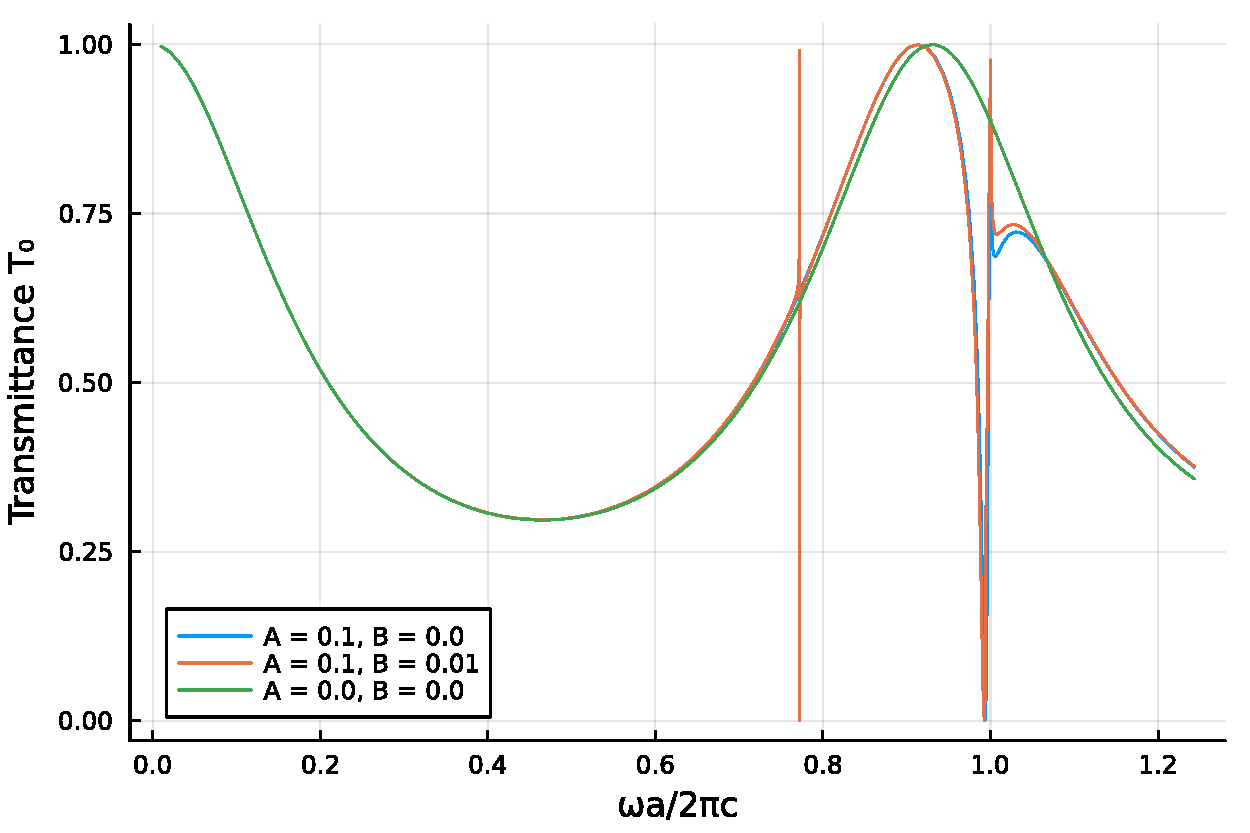
\includegraphics[width=0.6\columnwidth]{figures/ex4_bic_v1.pdf}
  \caption{Normalized angular frequency between 0 and 1.2.}
\label{fig:ex4_bic_v1}
\end{subfigure}
\begin{subfigure}{.5\textwidth}
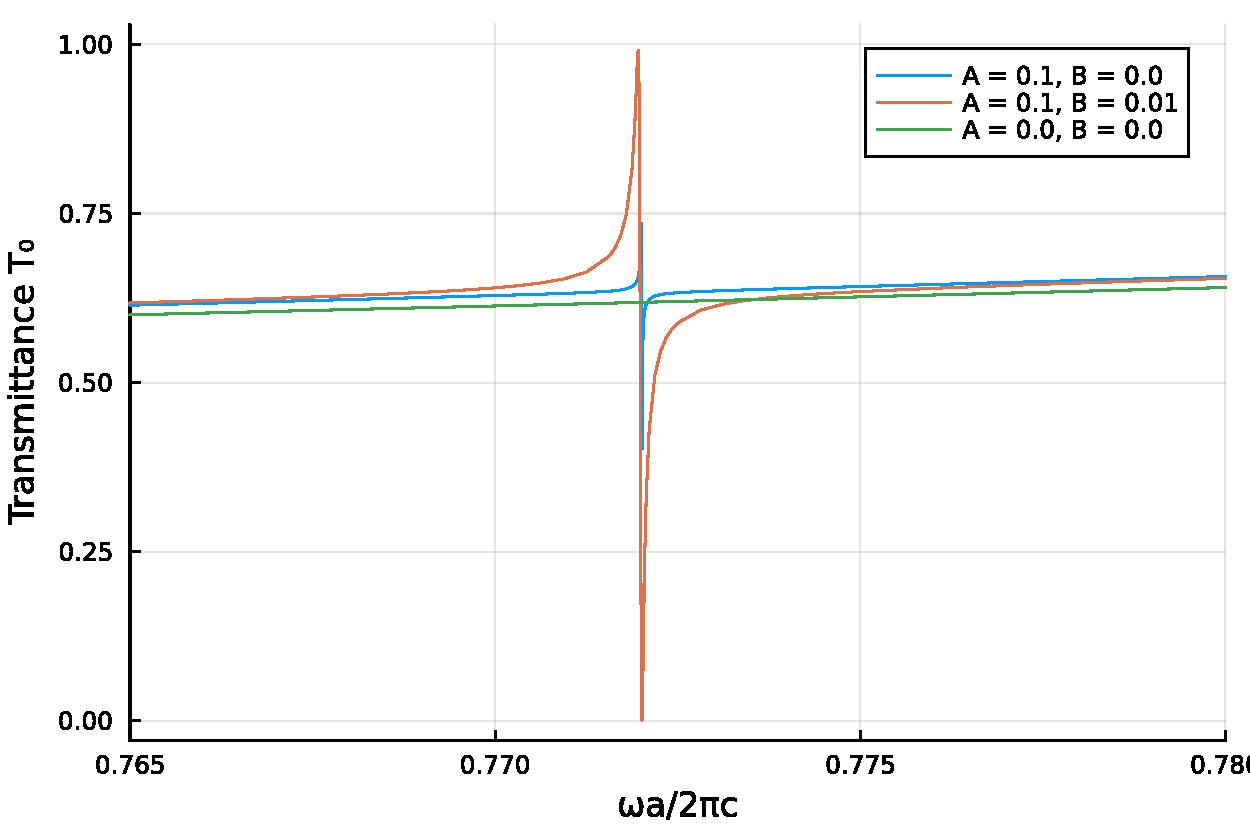
\includegraphics[width=0.6\columnwidth]{figures/ex4_bic_v2.pdf}
  \caption{Normalized angular frequency between 0.765 and 0.780.}
\label{fig:ex4_bic_v2}
\end{subfigure}
\begin{subfigure}{.5\textwidth}
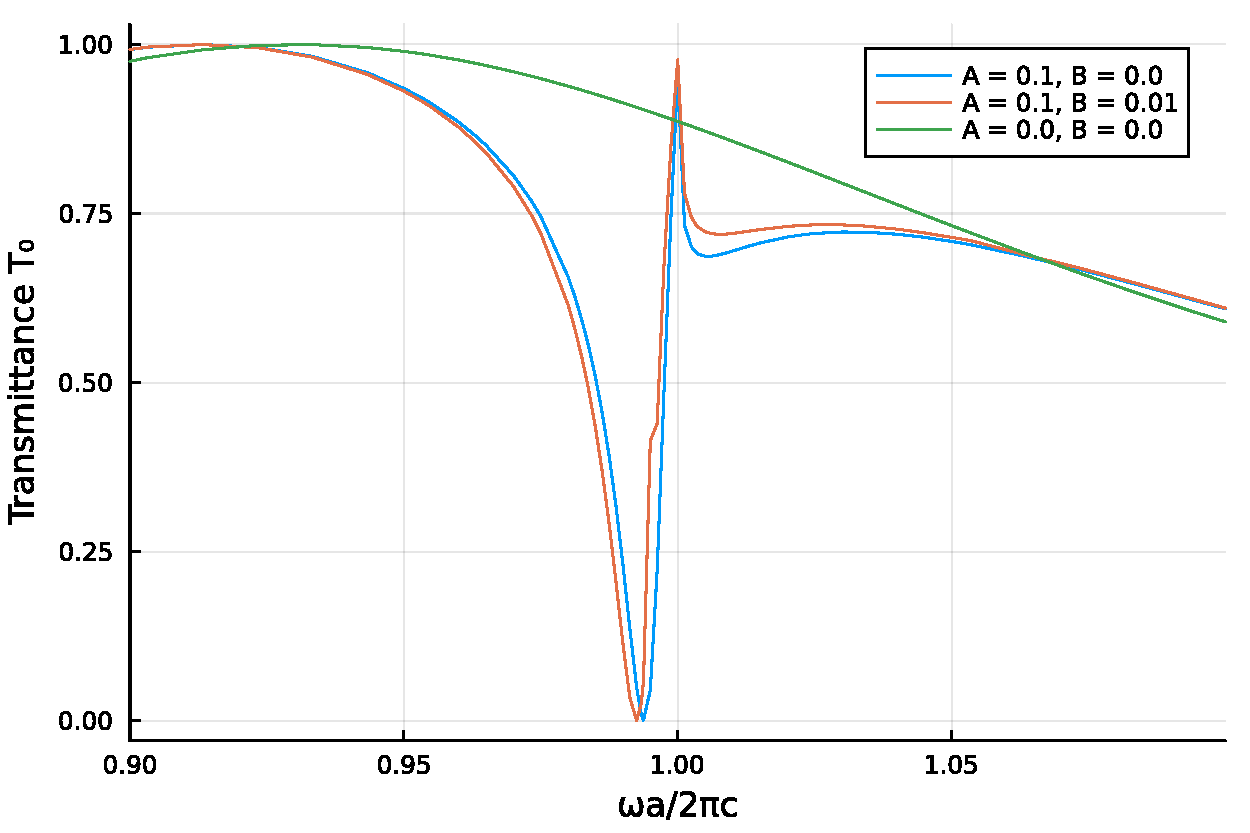
\includegraphics[width=0.6\columnwidth]{figures/ex4_bic_v3.pdf}
  \caption{Normalized angular frequency between 0.9 and 1.1.}
\label{fig:ex4_bic_v3}
\end{subfigure}
\caption{Third example. Transmittance of the zeroth-order diffraction as a function of normalized angular frequency, for various values of the sinusoidal amplitudes $A$ and $B$.}
\label{fig:ex4_bic}
\end{figure}

\subsection{Fifth example}
We consider a photonic crystal (PhC) slab consisting in 16 layers of infinite cylinders, separated by a distance of $L$, with a radius of $0.2$, and permittivity $\epsilon=8.9$, as depicted in \cref{fig:phc_multilayer}. If the PhC slab extended indefinitely towards the negative $y$-direction, then it would have a projected band diagram, which is shown in \cref{fig:phc_band}, where a bandgap (in yellow) is found approximately between the normalized frequencies $0.28$ and $0.45$. For our finite PhC slab, we plotted in \cref{fig:ex5_multiple_wl} the transmittance as a function of frequency, for normally incident light. The bandgap, where the transmittance drops abruptly to zero, is clearly seen around the normalized frequencies previously mentioned. 

\begin{figure}[h!]
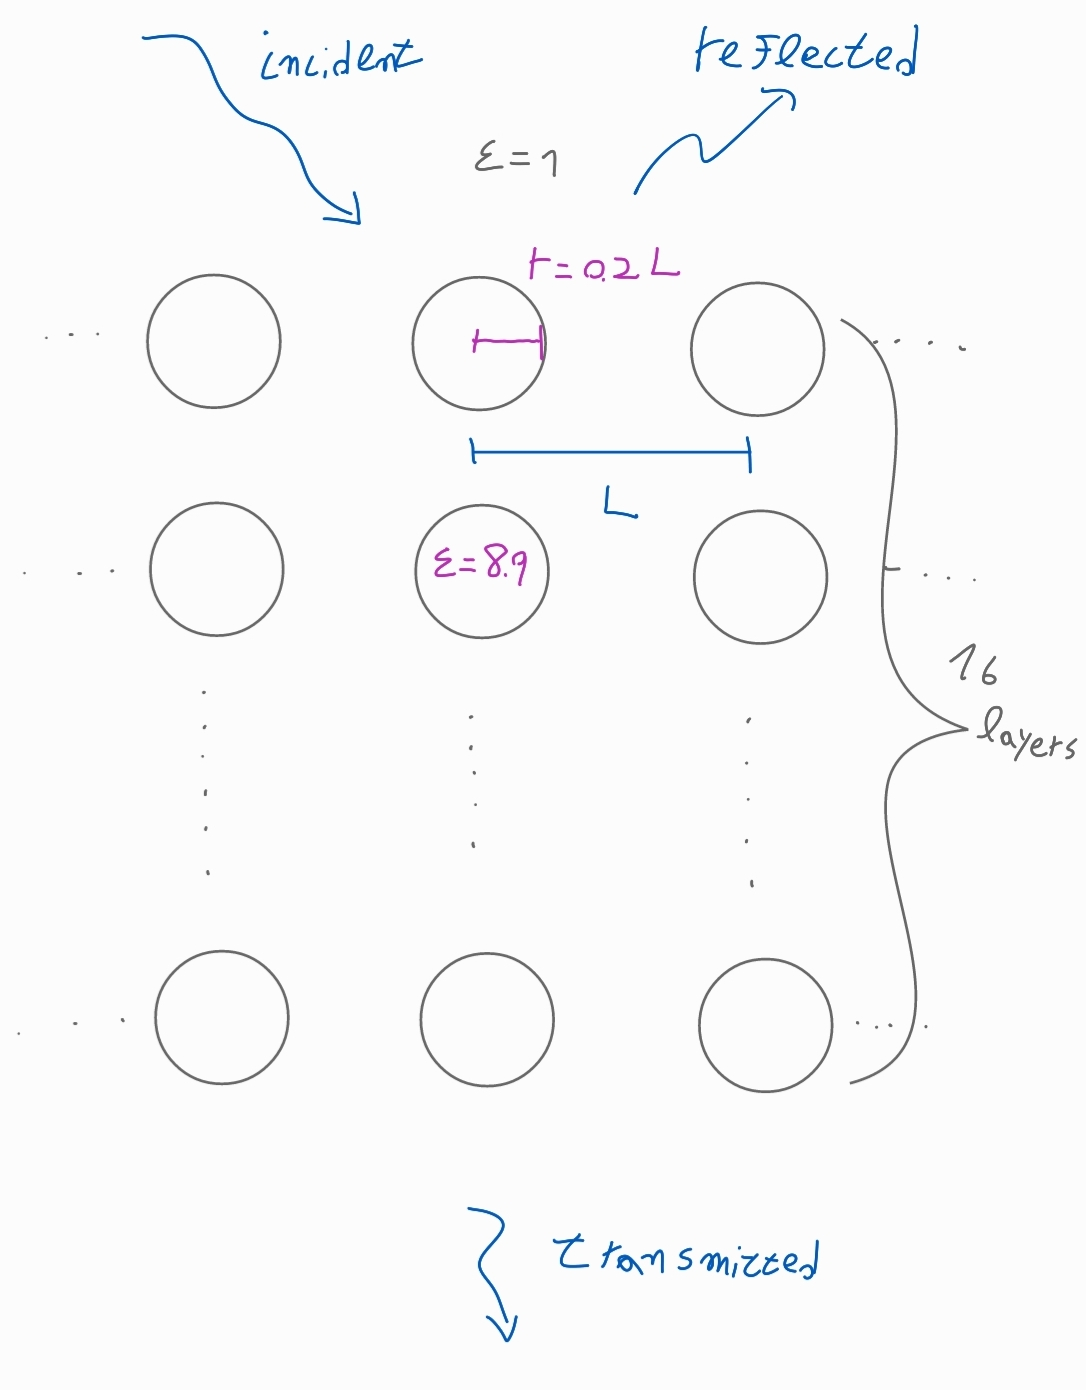
\includegraphics[width=0.4\columnwidth]{figures/phc_multilayer.jpg}
\caption{Fifth example. PhC slab comprising 16 layers of infinite cylinders of permittivity $8.9$, separation $L$ and radius $0.2L$.}
\label{fig:phc_multilayer}
\end{figure}

\begin{figure}[h!]
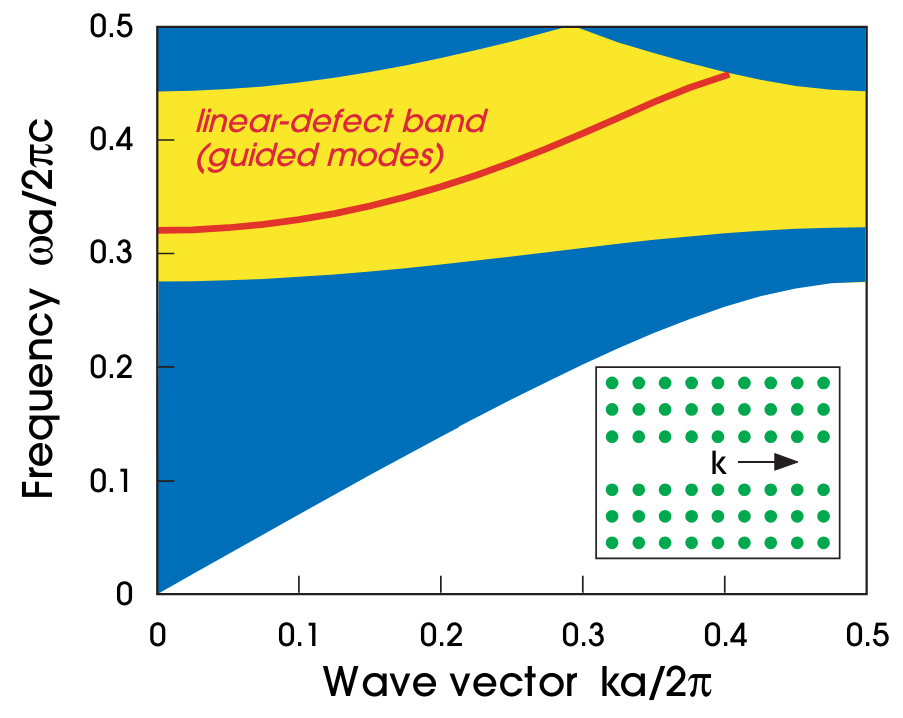
\includegraphics[width=0.6\columnwidth]{figures/phc_band.png}
\caption{Fifth example. Projected band diagram of the PhC shown in \cref{fig:phc_multilayer}, if it had an infinite extension in the $y$-direction. Obtained from \cite{joannopoulos2008molding}.}
\label{fig:phc_band}
\end{figure}

\begin{figure}[h!]
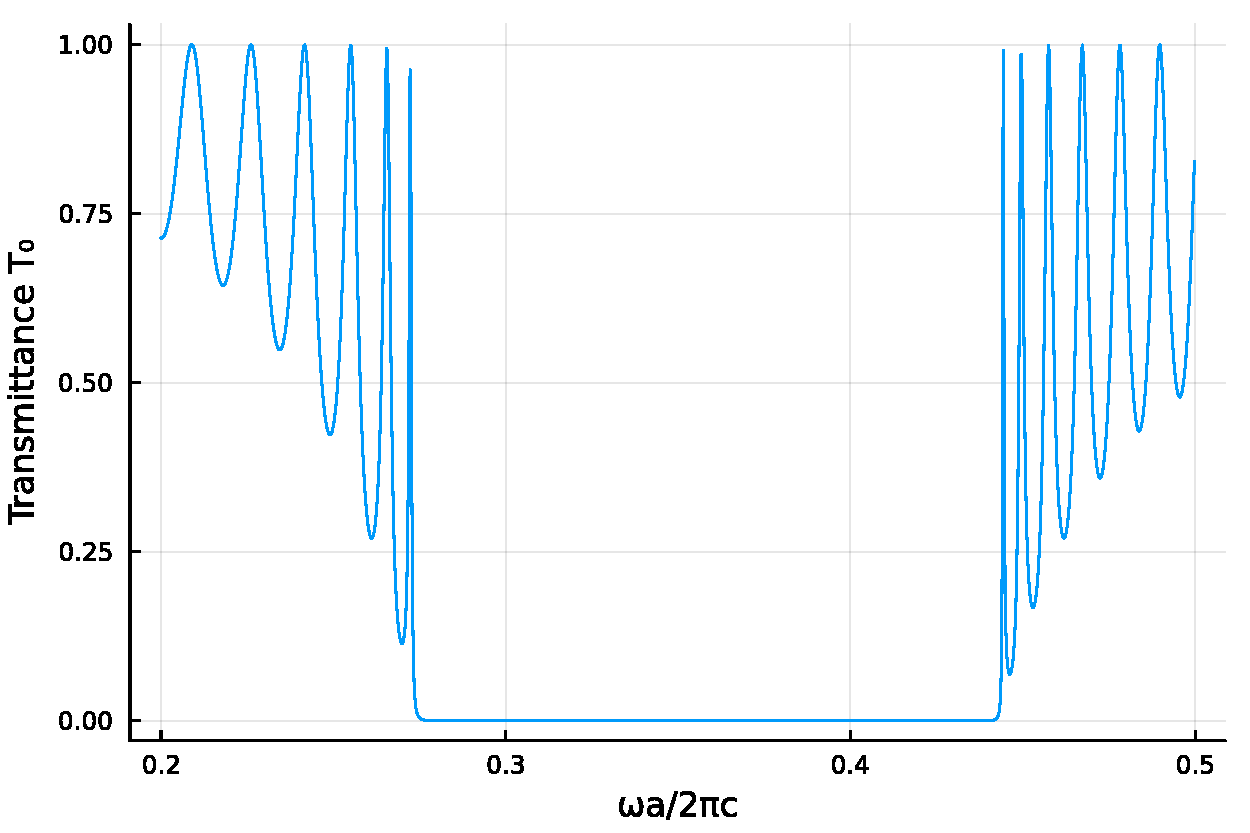
\includegraphics[width=0.6\columnwidth]{figures/ex5_multiple_wl.pdf}
\caption{Fifth example. Transmittance as a function of normalized angular frequency. A bandgap is clearly visible.}
\label{fig:ex5_multiple_wl}
\end{figure}

\subsection{Sixth example}
For our last example we consider a single row of our PhC slab, shown in \cref{fig:phc_singlelayer}, and we plot the condition number of the system matrix as a function of $\alpha_0$ (or equivalently as a function of the angle of incidence), for a fixed angular frequency of $\omega L / 2\pi c = 1.25$. This is shown in \cref{fig:ex5_cond_number}, where we have marked with a dashed line a Wood anomaly (where a new diffraction order emerges) at $\alpha_0 L / 2\pi = 0.25$. We first observe that the condition number of the system is high in all cases, being in the order of $10^6$. The fact that the BIE-NtD method yields ill-conditioned matrices was recognized by Lu and Lu \cite{lu2012high}, who proposed slight modifications to improve the conditioning of the resulting system. On the other hand, it is observed that, at the Wood anomaly, the condition number increases but remains in the same order of magnitude, which suggests that the BIE-NtD method could be robust at Wood anomalies.

\begin{figure}[h!]
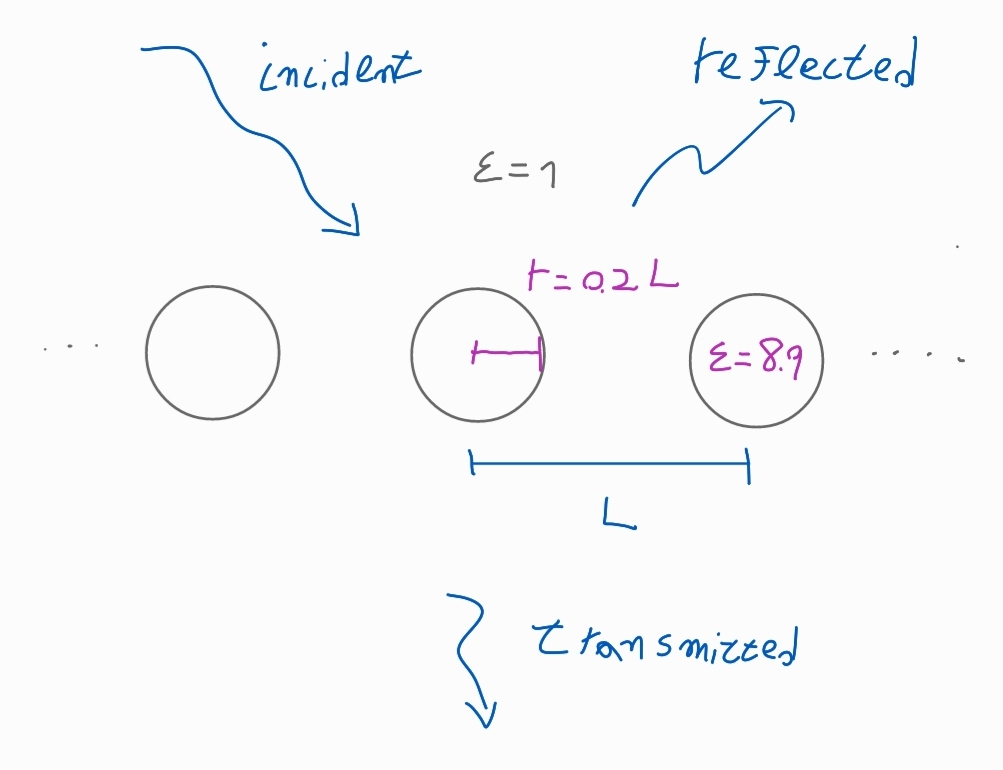
\includegraphics[width=0.6\columnwidth]{figures/phc_singlelayer.jpg}
\caption{Sixth example. A grating of a single row of cylinders.}
\label{fig:phc_singlelayer}
\end{figure}

\begin{figure}[h!]
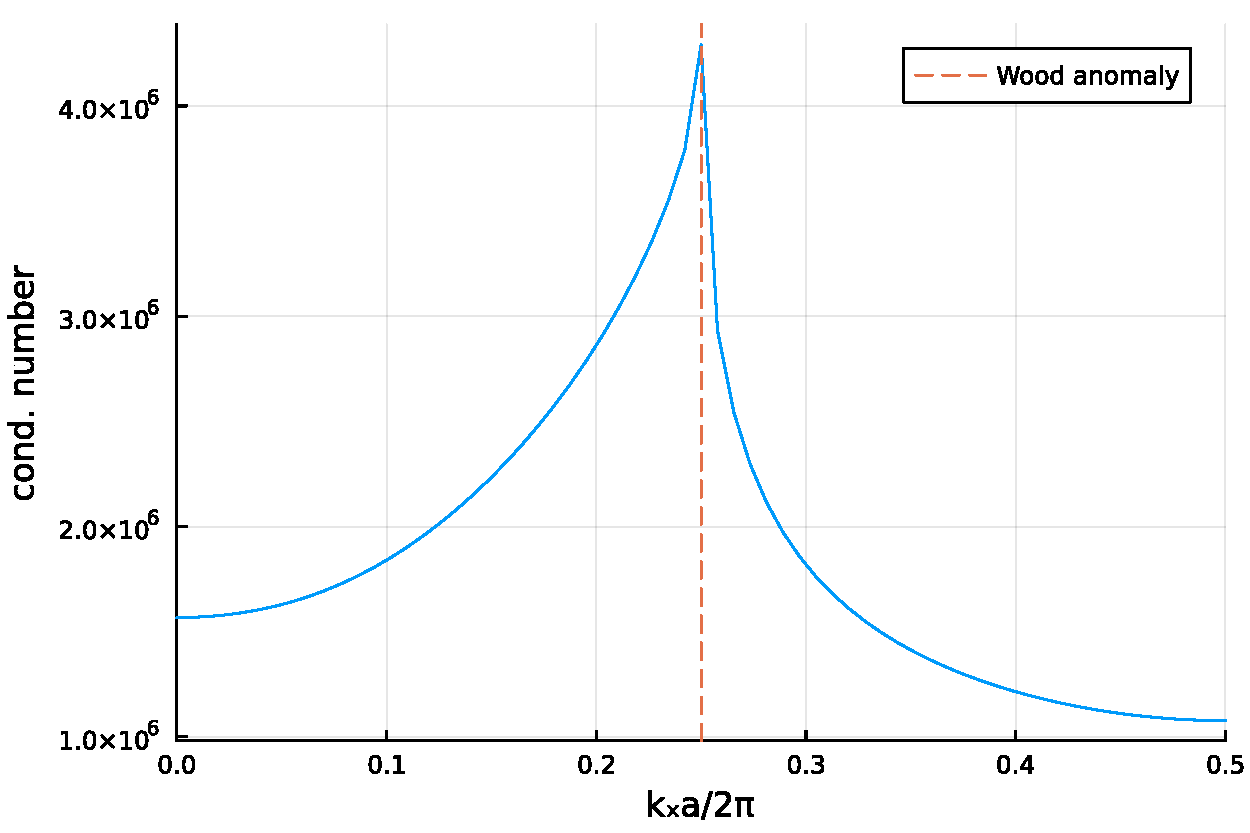
\includegraphics[width=0.6\columnwidth]{figures/ex5_cond_number.pdf}
\caption{Sixth example. Condition number of the resulting linear system as a function of the Bloch wavenumber (or angle of incidence), for a fixed normalized frequency of $\omega L / 2\pi c = 1.25$.}
\label{fig:ex5_cond_number}
\end{figure}


\section{Conclusion}
In this report we have explained the operation of the BIE-NtD method, proposed by Wu and Lu \cite{wu2009analyzing} for the computation of transmission and reflection coefficients of 1D-periodic diffraction gratings and PhC slabs. Additionally, we established an analogy of this method with the Transfer Matrix Method (TMM) for planar isotropic layered media, and recognized the BIE-NtD method as a direct generalization of the TMM for isotropic layered media with periodic interfaces. Finally, we have displayed various examples of interest employing the BIE-NtD method.

The BIE-NtD method, in its present state, is not efficient: it requires dense linear algebra operations, such as computing Schur complements, to solve the diffraction problem; this renders the overall methodology as slow and inapplicable for large and complicated settings. We believe that modifications could greatly improve the speed of the BIE-NtD. For example, we could avoid the use of Schur complements. This would increase the size of the resulting linear system, but it could be alleviated with the use of fast matrix-vector products schemes, such as the Fast Multiple Method \cite{greengard1987fast}, coupled with Krylov space iterative linear algebra solver, such as GMRES \cite{saad1986gmres}. Alternatively, well-formulated Domain Decomposition methods can also be employed. On the other hand, we checked that the BIE-NtD method yields ill-conditioned system matrices. This issue is corrected in the next iteration of the method, presented in \cite{lu2012high}.

%\begin{acknowledgments}
%\end{acknowledgments}

%\appendix

\bibliography{biblio}% Produces the bibliography via BibTeX.

\end{document}
